\section{Detector Infrastructure}
\label{sec:fdsp-tc-infr}


The  \dword{jpo} will provide the infrastructure needed to install the \dword{spmod}. The major items, described below, include the \dword{dss}, the electronics mezzanine on the cryostat roof (including racks), cable trays, an underground cleanroom with appropriate installation equipment, piping inside the cryostat, and \coldbox{}es with associated cryogenic supply. 

Other items, not described here but also in the \dword{jpo} scope, include a small machine shop, scissor lifts, rigging equipment, hand tools, diagnostic equipment (including oscilloscopes, network analyzers, and leak detectors), local storage with some critical supplies, and \dword{ppe}.  

%%%%%%%%%%%%%%%%%%%%%%%%%%%%
%\subsection{Detector Support System}
\subsection{Detector Support System}
\label{sec:fdsp-tc-infr-dss}

The \dword{dss} provides the structural support for the \dword{spmod} inside the cryostat.  
It also provides the necessary infrastructure to move the detector elements into place during
assembly. 
The \dword{dss} is a new design, quite different from the \dword{pdsp} \dword{dss}. It is described in some detail in this
section. 
The detector elements supported by the \dword{dss} include the \dwords{ewfc}, the \dwords{apa}, and the \dwords{cpa} with top and bottom \dword{fc} panels. The nominal load of the detector elements both dry (in air) and wet (under \dword{lar}) are shown in Table \ref{tab:installation-DSS-load}. The weights listed are the current design weights and do not include any margin for future design changes.  
The \dword{dss}, however, is designed so the weights can be doubled, and it would still meet the requirements of the design codes.  
Deformations would increase due to any increase in loads, and this effect should be evaluated.
\begin{comment}
\begin{dunetable}
[DSS Loads]
{l|c|cc|cc}
{tab:installation-DSS-load}
{The expected dry and wet stratic loads for the DSS.}
\multicolumn{2}{c}{} &  \multicolumn{4}{|c}{Dry Weight}\\ \toprowrule
\multicolumn{2}{c|}{} & \multicolumn{2}{c|}{Unit Weight} & \multicolumn{2}{c|}{Total Weight}  \\ \colhline

Detector Component &\# Units& (kg)&(lbs) & (kg) &(lbs)\\ \colhline
Detector Support Structure (DSS) (not in liquid) & 1 &NA&NA& 12318  & 27100 \\ 
\colhline
Anode Plane Assembly (Installed APA pair/No cables)& 75&1184 &2604 &88768  &195290\\ 
\colhline
Cathode Plane Assembly (CPA) & 100& 233 & 513 & 23331 & 51327 \\ 
\colhline
Top or Bottom Field Cage module (FC TB)& 400&149 & 328	 & 59679 & 131294\\ 
\colhline
CE Cables &750& 182 & 400 & 13636 & 30000\\
\colhline
Field Cage Endwall  & 8	&904 &	1989  & 7234 & 15914\\ 
\colhline
{\bf Total} &  & & & 204966 &	450925\\ 
\colhline
\toprowrule

\multicolumn{2}{c|}{} &  \multicolumn{4}{c}{Wet Weight}\\
\toprowrule
Detector Support Structure (DSS) (not in liquid) & 1 & NA & NA & 12318 & 27100 \\ 
\colhline
Anode Plane Assembly (Installed APA pair/No cables)&75& &0 & 0 &0\\ 
\colhline
Cathode Plane Assembly (CPA) & 100& 45 & 99 & 4520 & 9943 \\ 
\colhline
Top or Bottom Field Cage module (FC TB)& 400 & 68 & 150	& 27359 & 60191 \\ 
\colhline
CE Cables & 75 & & & 13636& 30000 \\
\colhline
Field Cage Endwall & 8 & 283& 	622& 2263 & 4978\\  
\colhline
{\bf Total} &  & & &60096	 &132211 \\ 
\colhline
\end{dunetable}
\end{comment}

\begin{dunefigure}[\threed model of the \dword{dss} ]{fig:DSS}
  {\threed model of the \dword{dss} showing the entire
  structure on the left along with one \dword{apa} row and one
  \dword{cpa}-\dword{fc} row at each end. The right panel is a zoomed image
  showing the connections between the vertical supports and the
  horizontal I-beams.}
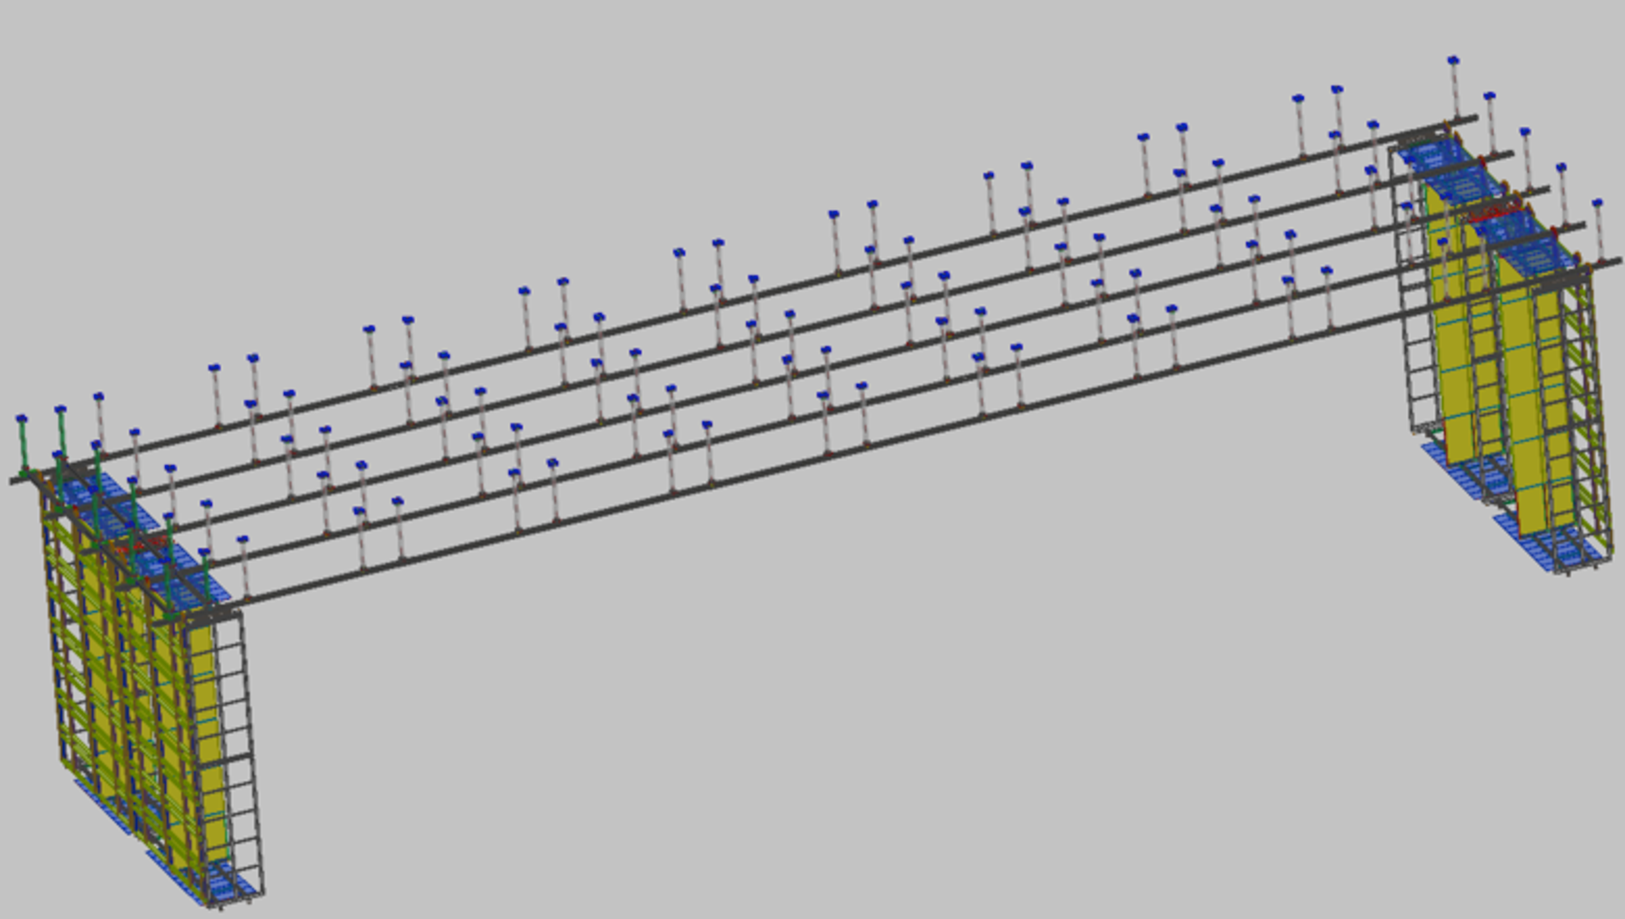
\includegraphics[width=.49\textwidth]{DSS-1.pdf}
 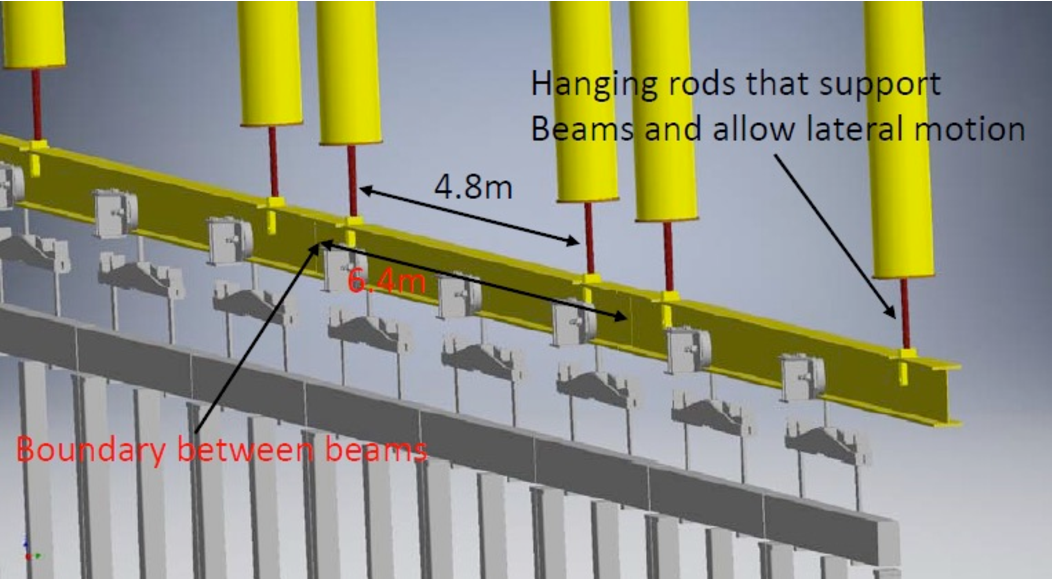
\includegraphics[width=.49\textwidth]{DSS-2.pdf}
\end{dunefigure}

The \dword{dss} is supported by the
cryostat outer steel structure through a series of \fdth{}s that cross through the cryostat insulation and anchored with flanges on
the cryostat roof. 
Inside the cryostat, a series of stainless steel I-beams are connected to the \fdth{}s and used to support the
detector. 
The \dword{dss} defines the location of the detector inside the cryostat and also defines how the detector elements move and contract as the detector is brought to \dword{lar} temperature. 
The design of the \dword{dss} encompasses the overall
structural design of the \dword{detmodule} because only after the elements are mounted to the \dword{dss} and connected do they make a unified mechanical structure. 
Figure~\ref{fig:DSS} (left) shows the \dword{dss} structure; there are
five rows of supports for the alternating rows of
\dword{apa}-\dword{cpa}-\dword{apa}-\dword{cpa}-\dword{apa}.  
The \dword{dss} is connected to the cryostat warm structure at a flange mounted on the outside of the cryostat.  
Figure~\ref{fig:DSS} (right)
shows the layout of these structural \fdth{}s.

The \dword{dss} is designed to meet the following  requirements:
\begin{itemize}
 \setlength\itemsep{1mm}
\setlength{\parsep}{1mm}
\setlength{\itemsep}{-5mm}
% \small
\item Support the weight of the detector;
\item Accommodate cryostat roof movement during filling, testing, and operation;
\item Accommodate variation in \fdth locations and
  variation in the flange angles due to installation tolerances and
  loading on the warm structure;
\item Accommodate shrinkage of the detector and \dword{dss} from ambient
  temperature to \dword{lar} temperature;
\item Define the positions of the detector components relative to each other; 
\item Provide electrical connection to the cryostat ground and remain electrically isolated from the detector;
\item Allow support penetrations to be purged with gaseous argon to prevent contaminants from diffusing back into the liquid; 
\item Ensure that the instrumentation cabling does not interfere with the \dword{dss};
\item Consist entirely of components that can  
be installed through the \dword{tco};
\item %Design to m
Meet AISC-360 or appropriate codes required at \dword{surf};
\item %Design to m
Meet seismic requirements one mile underground at \dword{surf};
\item Consist entirely of %All materials must be 
materials compatible for operation in ultrapure \dword{lar};
\item Ensure that beams are completely submerged in \dword{lar};
\item Ensure that detector components are not less than \SI{400}{mm} from the membrane flat surface;
\item Ensure that the supports do not interfere with the cryostat I-beam structures;
\item Ensure %Design such 
that the detector's lower \dword{gp} is lies over the cryogenic piping and that the tops of the \dword{dss} beams are submerged in \dword{lar} while leaving a \SI{4}{\%} ullage at the top of the cryostat;
\item Include the infrastructure necessary to move the \dword{apa} and
  \dword{cpa}-\dword{fc} assemblies from outside the cryostat through the
  \dword{tco} and to the correct position.
\end{itemize}

  The \dword{dss}
consists of pairs of \fdth{}s that support \SI{6.4}{m}-long
W10x26 stainless steel I-beam sections. The proposed design of the
\dword{dss} has \num{10} I-beam segments per row for a total of
\num{50} I-beam segments. Each I-beam is suspended on both ends by
rods from \fdth{}s that penetrate the cryostat roof.  %In the cold condition
When cold, each I-beam shrinks, causing gaps to form between
\dword{apa}s that are adjacent but supported on separate beams.
\dword{apa}s that are supported on the same beam will not have gaps
develop because both the beam and \dword{apa}s are stainless steel so
they shrink together.  Each beam is supported by a nearly
\SI{2}{m} long rod that allows the beam support to move as the beam
contracts.


The feedthrough consists of a flange and $6 ^{''}$ OD structural tube welded to it that extends through the cryostat insulation.  
There is a
nominal \SI{10}{mm} gap between the OD of the tube and the ID of the clearance tube in the cryostat. \fixme{OD and ID are not defined in the common glossary.}
The $6 ^{''}$ tube provides lateral support to the I-beams during installation.
Running down the center of the feedthrough is a $1^{"}$ diameter rod supported at a swivel washer at the flange and then supported by the
I-beam at a clevis.  The gas seal is obtained by Conflat Flange and a
bellows that seals around the swivel washer.  The lateral position and height of the rod can be adjusted $\pm$1 inch to accommodate tolerances in positioning cryostat crossing tubes. Figure \ref{fig:DSS-lateral-support} shows the end of the $6 ^{''}$ tube and how it locks the I-Beam into position. 

\begin{dunefigure}[DSS support for lateral loads ]{fig:DSS-lateral-support}
  {Left panel shows how the central support rod is locked in postion during detector installation. The outer $6 ^{''}$ tube is used to fix the support clevis in position. The right panel shows the system as it is connected to the I-Beam.}
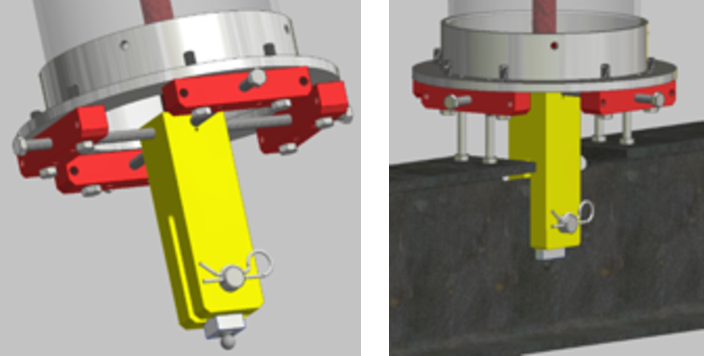
\includegraphics[width=.75\textwidth]{graphics/dss-lateral-support.pdf}
\end{dunefigure}

After the detector has been installed all restraints will be released to allow motion as the detector contracts during cool down.  The two hangars that support each \dword{dss} beam will contract and move toward each other by 13.1 mm along the axis of the detector.  
The drift distance will shrink by 7.4mm caused by the contraction of the field cages.  The detector is symmetric in the drift direction around the center \dword{apa}.  The drifts on either side of the center \dword{apa} will  shrink toward the center while the center \dword{apa} remains unmoved.  This results in the \dwords{cpa} moving 7.4mm toward the center and the outer \dword{apa}s moving 14.8mm (2*7.4mm) toward the center.  The hanging rod is designed to have a range of motion of 15mm in the drift direction to accommodate this shrinkage.




Detector components are installed using a shuttle beam system as
illustrated in Figure~\ref{fig:shuttle}.  
The last two columns of
\fdth{}s (eastern-most) support temporary beams that run
north-south, perpendicular to the main \dword{dss} beams.  
A shuttle beam has trolleys mounted to it and transverses 
north-south until it aligns with the required row of \dword{dss} beams.  
The last \dword{apa} or \dword{cpa} in a row is supported by the shuttle beam, which is bolted directly to the \fdth{}s once it is in place.  
As the last \dword{cpa} or \dword{apa} in each row is installed, the north-south beams are removed.

\begin{dunefigure}[\threed models of the shuttle beam end of the \dword{dss}]{fig:shuttle}
  {\threed models of the shuttle beam end of the \dword{dss}. The figures show how an \dword{apa}
is translated into position using the north-south beams until it lines up with the correct
row of I-beams.}
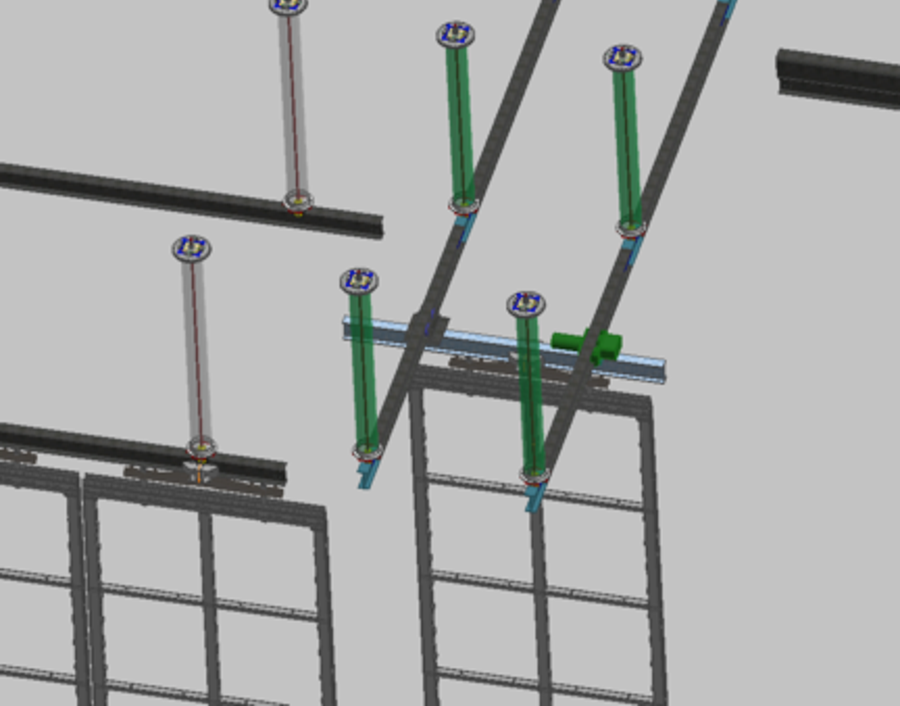
\includegraphics[width=.49\textwidth]{/Shuttle-1.pdf}
 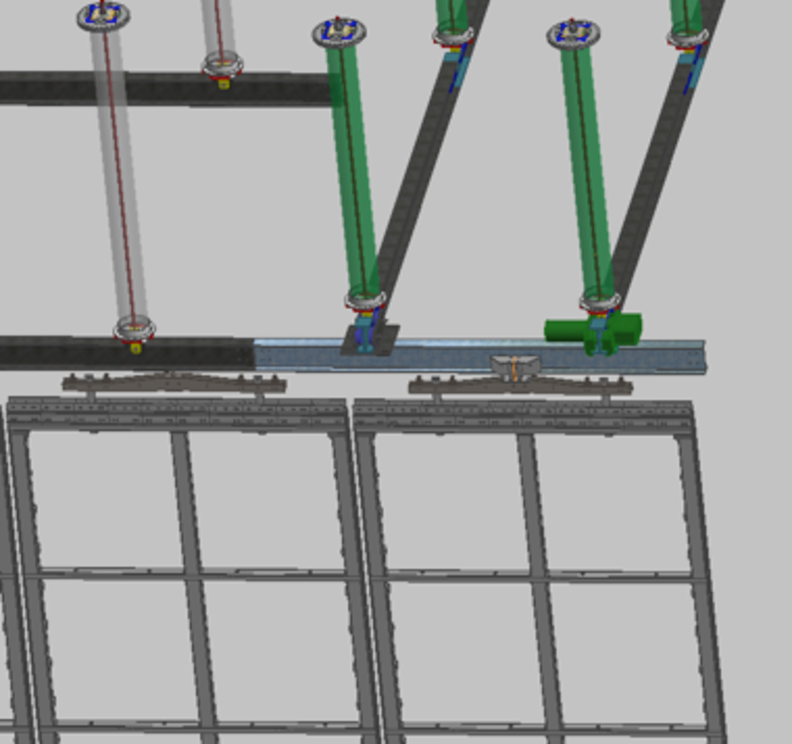
\includegraphics[width=.42\textwidth]{shuttle-2.pdf}
\end{dunefigure}

A mechanical interlock system  prevents trolleys
from passing the end of the shuttle beam unless it is aligned with a
corresponding \dword{dss} beam.  The shuttle beam and each detector component are
moved using a motorized trolley.  A commercially available motorized
trolley will be modified as needed for the
installation. 




\begin{dunefigure}[Prototype of the motorized DSS trolley ]{fig:DSS-trolley}
  {Prototype of the motorized DSS trolley that will push the APA and CPA along the I-beams and through the switchyard.}
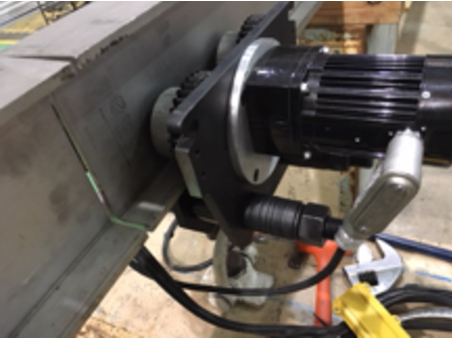
\includegraphics[width=.49\textwidth]{graphics/DSS-trolley.pdf}
\end{dunefigure}



A mock-up of the shuttle system will be constructed to test the
mechanical interlock and drive systems for the shuttle beam
for each \dword{detmodule}.  Tests will be conducted to evaluate the level of
misalignment between beams that can be tolerated and the amount of
positional control that can be achieved with the motorized trolley. We plan to construct a full scale prototype of a section of the  switchyard and perform tests at floor level. Later, the test program will be expanded at Ash River, where a full scale installation test will be performed. This is described in the installation \dword{qa} section.


%%%%%%%%%%%%%%%%%%%%%%%%%%%%
\subsection{Cryostat Roof Infrastructure}
\label{sec:fdsp-tc-infr-cryo-roof}

\begin{dunefigure}[Mezzanine and electronics racks]{fig:mezzanine}
  {The electronics racks sit on the \dword{dune} electronics mezzanine as shown. The top image is a view from above the detector looking at the racks from the side. In this view the cavern and cryogenics mezzanine are hidden. The bottom view is from the end of the cryostat looking over the roof. Here, the access stairs to the mezzanine are shown.}
 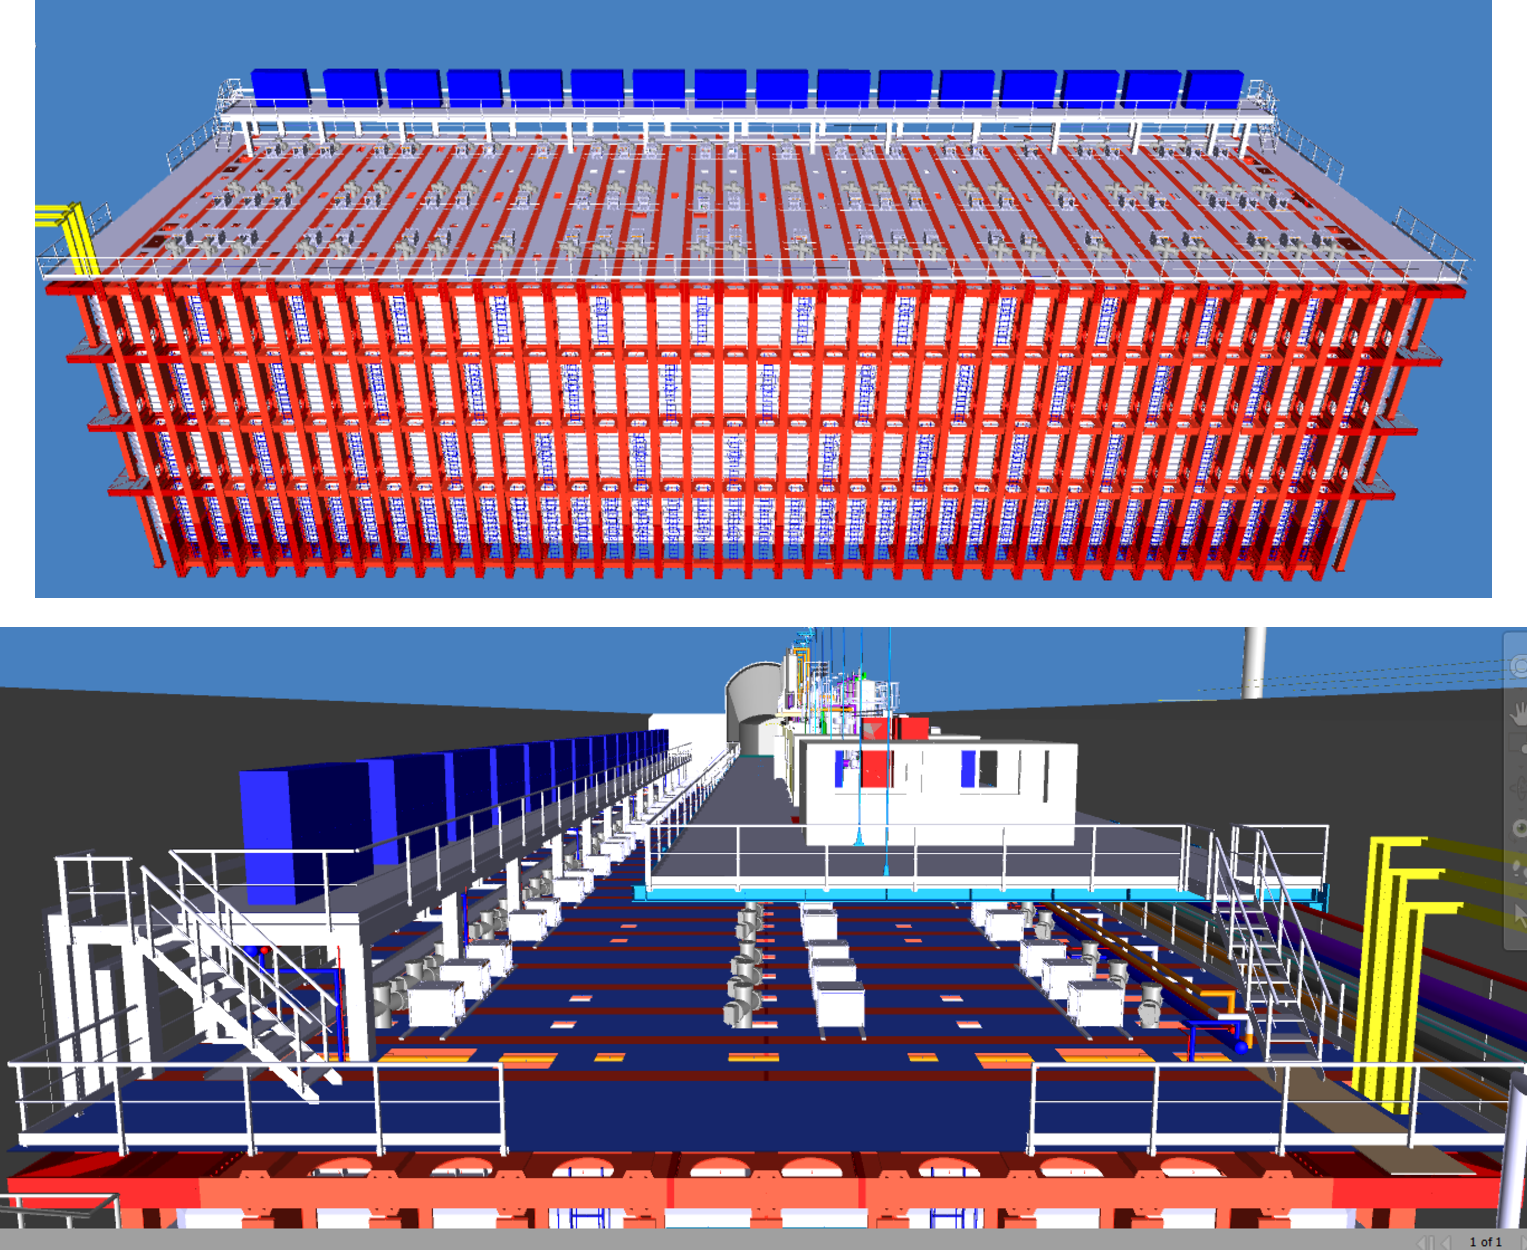
\includegraphics[width=\textwidth]{mezzanine.pdf}
\end{dunefigure}

\begin{dunefigure}[Electronics rack contents]{fig:rack-build1}
  {The nominal contents of the electronics racks on the mezzanine is shown. Each rack is configured to consume less than 3.5 \si{kW}. }
 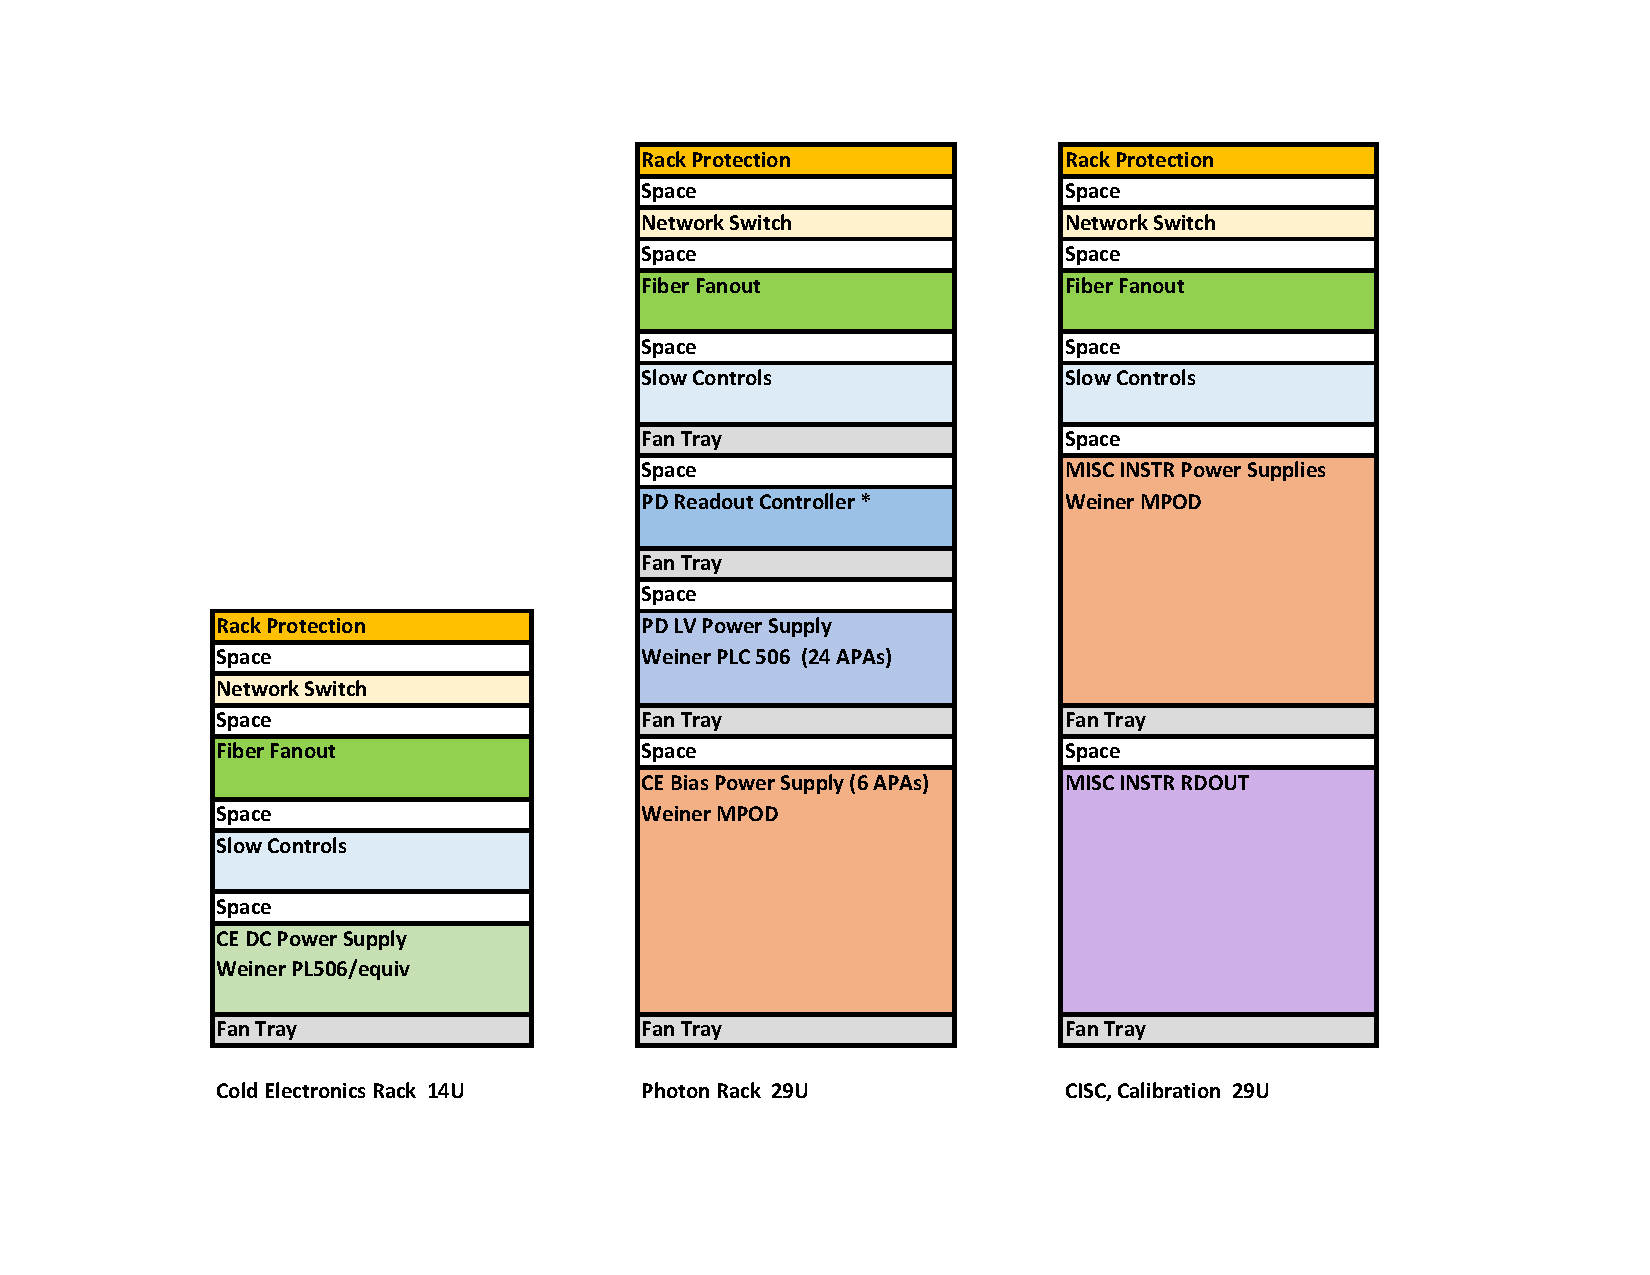
\includegraphics[width=.8\textwidth]{rack-build1} %pdf} It had too much room around it (was at .98)
\end{dunefigure}

The top image in Figure \ref{fig:mezzanine} shows the \dword{dune} electronics mezzanine with the 42U tall racks placed on top. 
During the initial design steps, it became clear that the constraints placed on the rack location by the many \dword{dss} support \fdth{}s, the electronics \fdth, and the I-beams themselves make distributing the racks on the roof very challenging. 
By constructing a fixed mezzanine for the electronics above the cryostat at the same height as the cryogenic mezzanine, the electronics \fdth{}s are kept clear. 
This configuration also makes working on the electronics much easier because there are no local obstacles and all the racks are in one place.

As the electronics modules in the  racks are connected to the detector readout electronics they are by definition at detector ground so the mezzanine must also be connected to detector ground, which is accomplished by bolting the mezzanine to the cryostat I-beams. 
 
Figure \ref{fig:mezzanine} (top) shows 16 groups of five racks each
on the mezzanine for a total of 80 racks. 
The electronics inside the detector racks will be air cooled and the heat rejected into the cavern air. 
If the cavern temperature increases beyond an acceptable level due to the electrical heating then water cooled heat exchangers can be added to the racks. \dword{cf} will provide sufficient chilled water capacity at the entrance to the north cavern to accommodate the maximum heat load. 
The major heat load resides with the cold electronics and photon electronics located near the cryostat \fdth{}s which is difficult to water cool. 
The cooling capacity of the cavern air conditioning system roughly matches the expected heat generation by the electronics modules for one detector so it is not expected to need the additional chilled water capacity until detector \#3 is installed. 
At this time either the racks can be switched to chilled water cooling or the chilled water can be used for an additional air handling unit in the cavern.


Of the 80 racks, \dword{ce} \dword{lv} power require \num{25}, and another 25 will be made available collectively for  \dword{apa} wire bias voltage, \dword{pd} power and miscellaneous additional \dword{ce}, \dword{pds}, and  \dword{apa} electronics modules. 
The remaining 30 will be available for slow control, calibration, and other electrical equipment. 
Small 12U high mini-racks will  be placed near the electronics \fdth{}s for the \dword{pd} readout electronics and optical patch panels. If this is not enough, additional racks can be placed on the cryostat roof. The present rack configuration for this layout is shown in Figure~\ref{fig:rack-build1}. 
The electronics modules inside the racks are distributed to keep power consumption for each rack below \SI{3.5}{kW}. 
The racks are 42U high, which provides significant extra rack space.  If the \dword{ce} requires additional electronics, however, the items would need to go in a \dword{pd} rack to respect the per-rack power limit.

The 12U high mini-racks near the \fdth flanges will be relatively empty because the \dword{pd} readout should need only approximately 2U in height while the \dword{ce} patch panel needs less than 1 U. The mini-racks are shown in the lower panel of Figure \ref{fig:mezzanine}; 
they are the gray rectangles near the electronics crosses.

The north-south cable trays (transverse to the beam) which run from the electronics mezzanine to the electronics \fdth are routed under the floor of the cryostat roof (shown in gray in Figure \ref{fig:mezzanine}) next to the 
I-beams. 
This keeps the roof reasonably clear, so that equipment can be transported across it.
The gap between the web of the I-beams is \SI{1.2}{m} so 
a \SIrange{200}{300}{mm} wide cable tray installed along the beams 
leaves enough space for people to work on the electronics crates while standing directly on the cryostat's outer steel skin (Figure \ref{fig:install-elect-cross}). 
The cable trays between the \dword{cuc} and the electronics mezzanine will run along the west end of the cryostat under the floor of the cryostat roof. 
We estimate only half of the \SI{1.6}{m} space is needed, so the cable tray quantity could in principal be doubled if necessary. 

The flooring material for the \dword{spmod}
will be similar to the \SI{25}{mm} thick plywood used at \dword{pdsp}. 
It must be easy to cut so as to fit around many obstacles and pipes on the roof, it must be light enough to lift up to allow access under the floor, and it must support the load of a person and a small cart. 
We will investigate fire-retardant options available in the USA, with input from the \dword{fnal} fire life-safety group. 

Air filters for the cleanroom and inside the cryostat will also be placed on the cryostat roof. The present plan is to place fan filter units near the manholes on the east end of the cryostat. Initial calculations indicate sufficient airflow is possible to support one air exchange per hour inside the cryostat. The air handling system has yet to be designed in detail.


\begin{dunefigure}[Cryostat crossing tube design]{fig:crossingtube}
  {Draft drawing of the cryostat crossing tubes. The hatched region is the cryostat insulation. Units are mm. Points labeled ``u'' and ``v'' are welds. }
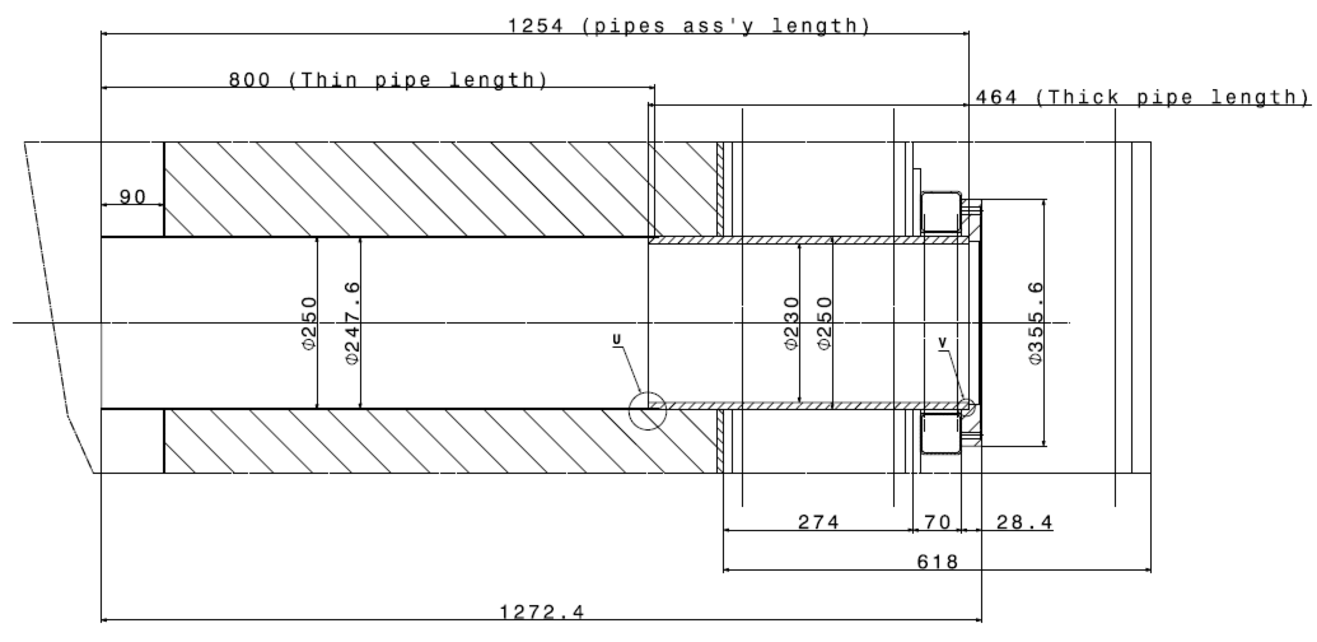
\includegraphics[width=.85\textwidth]{crossingtube}
\end{dunefigure}
 
The cryostat crossing tubes are among the most critical components of the roof infrastructure since they penetrate the cryostat roof and connect to the cold cryostat membrane. The top flange of the crossing tube supports either the electronics \fdth or the detector support \fdth and must be directly tied to the steel I-beams for support. 
Accurate placement and true vertical installation of the crossing tubes is important to ensure proper interfacing to the cryostat membrane. 
A draft assembly drawing of the crossing tube is shown in Figure~\ref{fig:crossingtube}. 
The crossing tube consists of a \SI{464}{mm} long stainless steel pipe with a \SI{1}{cm} thick wall. 
One end of the thick walled section is welded to a \SI{800}{mm} long \SI{250}{mm} diameter thin walled tube which is also welded to the cryostat membrane.
A custom Conflat flanges at the top end of the crossing tube connects to the \fdth. 
The thick tube section is also welded to the steel roof plates (the thin cross-hatched segments in Figure~\ref{fig:crossingtube}).  


%To ensure that the crossing tubes are adequately cleaned during the initial gaseous argon (\dword{gar}) purge and that air is removed from the tubes, each crossing tube has a small side port connected to a network of pipes on the roof of the cryostat. During the initial \dword{gar} purge, argon gas is withdrawn from each port and analyzed to assess progress and determine when the system is ready to be cooled down. The large number of crossing tubes, about 250 in the \dword{sp} configuration, means the content from each port cannot be analyzed independently of all others. Five streams, each one collecting gas from about 50 crossing tubes are connected independently to the gas analyzers. Gas impurities accumulate in the ullage. During steady state operations, \dword{gar} from the crossing tubes will be analyzed to ensure that impurities are adequately removed from the \dword{gar}.    If additional cleaning of the ullage is necessary, the \dword{gar} withdrawn from all ports, or a smaller set of them, can be sent to the condenser, re-condensed, and purified in the liquid phase along with the rest of the \dword{lar}. To detect any possible leaks that could develop in the room temperature feedthroughs over time, simple O$^2$\ sensors monitor the return gas for traces of oxygen, which would indicate a leak.
 
Each or the 250 crossing tubes has a small side port which connects to the cryogenic gas handling system through a network of pipes on the cryostat roof. During the initial \dword{gar} purge,  \dword{gar} is withdrawn from each port and analyzed to assess progress and determine when the system is ready to be cooled down. Five \dword{gar} streams, each collecting gas from 50 crossing tubes, are connected independently to the gas analyzers. This provides some redundancy and position dependant information on the contamination level of the gas a the top of the cryostat during the purge.
 
During filling and normal operation the collection and analysis of the gas from the crossing tubes will continue to ensure that impurities, which are generated in the cables in the \fdth{}s or the warmer surfaces in the ullage,  are adequately removed from the \dword{gar}. If the gas analyzers find no significant nitrogen contamination, the \dword{gar} from all or a subset of ports can be sent to the condenser, re-condensed, and purified along with the rest of the \dword{lar}. Simple O$_2$\ sensors monitor the return gas for traces of oxygen, which would indicate development of a leak in the room temperature \fdth{}s.

Each detector has a power budget of \SI{500}{kVA}. The total power budget available for use by detector electronics is derated to \SI{400}{kW} at the power distribution panels.  The \dword{ce} is the detector's largest power consumer.  
The \dword{ce} dissipates \SI{306}{W} per \dword{apa}.  
The \dword{lv} power supplies' controller needs about \SI{35}{W} per \dword{apa} and has an efficiency of approximately 85 percent. This leads to an approximately  \SI{400}{W} load per \dword{apa}, or a total load of  \SI{60}{kW} per \dword{detmodule}.  The \dword{apa} wire-bias power supplies have a maximum load of  \SI{465}{W} per set of six \dword{apa}s, for a total budget of around  \SI{12}{kW}.   Cooling fans and heaters near the \fdth{}s will use a nominal amount of power, so the overall power budget for \dword{ce} and  \dword{apa}
is expect to be less than \SI{75}{kW}.


The \dword{pds} electronics is based on the Mu2e electronics, which reports a power load of approximately  \SI{6}{kW}.  \dword{dune} plans a power budget of  \SI{8}{kW} because of cable drops and  power supply inefficiencies.  

Each of the approximately 80 detector racks will have fan units, Ethernet switches, rack protection, and slow controls modules, adding a load of about \SI{500}{W} per rack, for a total of \SI{40}{kW}.

Twenty-five racks are reserved for cryogenics instrumentation with a per-rack load conservatively estimated at \SI{2}{kW}, for a total of \SI{50}{kW}. 

The \dword{detmodule} will thus use  an estimated \SI{173}{kW} of power.   These numbers provide a safety factor of about two on our power estimates relative to available power.


%%%%%%%%%%%%%%%%%%%%%%%%%%%%
\subsection{Cryostat Internal Infrastructure}
\label{sec:fdsp-tc-infr-cryo-int}

%%%%Internal Cryogenics%%%%
\label{sec:fdsp-tc-internal-cryo}

The internal cryogenics comprises three sets of pipe distribution networks and two sets of sprayers. All pipes enter the cryostat from the top; some go all the way down to the floor, and others remain in the ceiling. On the floor are
\begin{itemize}
\setlength\itemsep{1mm}
\setlength{\parsep}{1mm}
\setlength{\itemsep}{-5mm}
\item \textbf{GAr distribution}: a set of pipes flowing GAr. These pipes are used only at the beginning to remove air that fills the cryostat. They have either a longitudinal slit or calibrated holes to distribute GAr uniformly along the length of the cryostat. Computational fluid dynamics simulations show that air will be removed from the system as long as GAr is flowing in at the right speed, calculated and experimentally verified as \SI{1.2}{m/hr}.


\item \textbf{\dword{lar} distribution}: two sets of pipes flowing \dword{lar}. These pipes are used to fill the cryostat and, during steady state operations, to return the \dword{lar} from the purification system. The pipes have calibrated holes to return the \dword{lar} uniformly throughout the length of the cryostat. This is very important for uniform purity. Four pumps circulate the \dword{lar}. Initially, all of pumps operate at once to achieve purity, but once the target purity is achieved, only one or two pumps remain in service. Two sets of pipes are needed to adequately distribute the \dword{lar} over this broad range of flow rates.
\end{itemize}

On the ceiling are

\begin{itemize}
\setlength\itemsep{1mm}
\setlength{\parsep}{1mm}
\setlength{\itemsep}{-5mm}
\item \textbf{Cool down sprayers}: Two sets of cool down sprayers are distributed along the long sides of each cryostat. One set distributes \dword{lar} using liquid sprayers that generate a conical profile of small droplets of liquid. The other set of sprayers distributes GAr to move the \dword{lar} droplets inside and cool down the detector and cryostat uniformly. These sprayers are being tested in \dword{pddp}. They are a variation of those implemented in \dword{pdsp}.
\end{itemize}

Figure~\ref{fig:internal-cryo-3D} shows the current layout of the internal cryogenics. 
%The current drawing of the internal cryogenics is presented in Figure~\ref{fig:internal-cryo-drawing}. 
The GAr pipes are in red, the \dword{lar} pipes in blue.

\begin{dunefigure}[Cryogenic piping inside the cryostat ]{fig:internal-cryo-3D}
  {Layout of the internal cryogenics.}
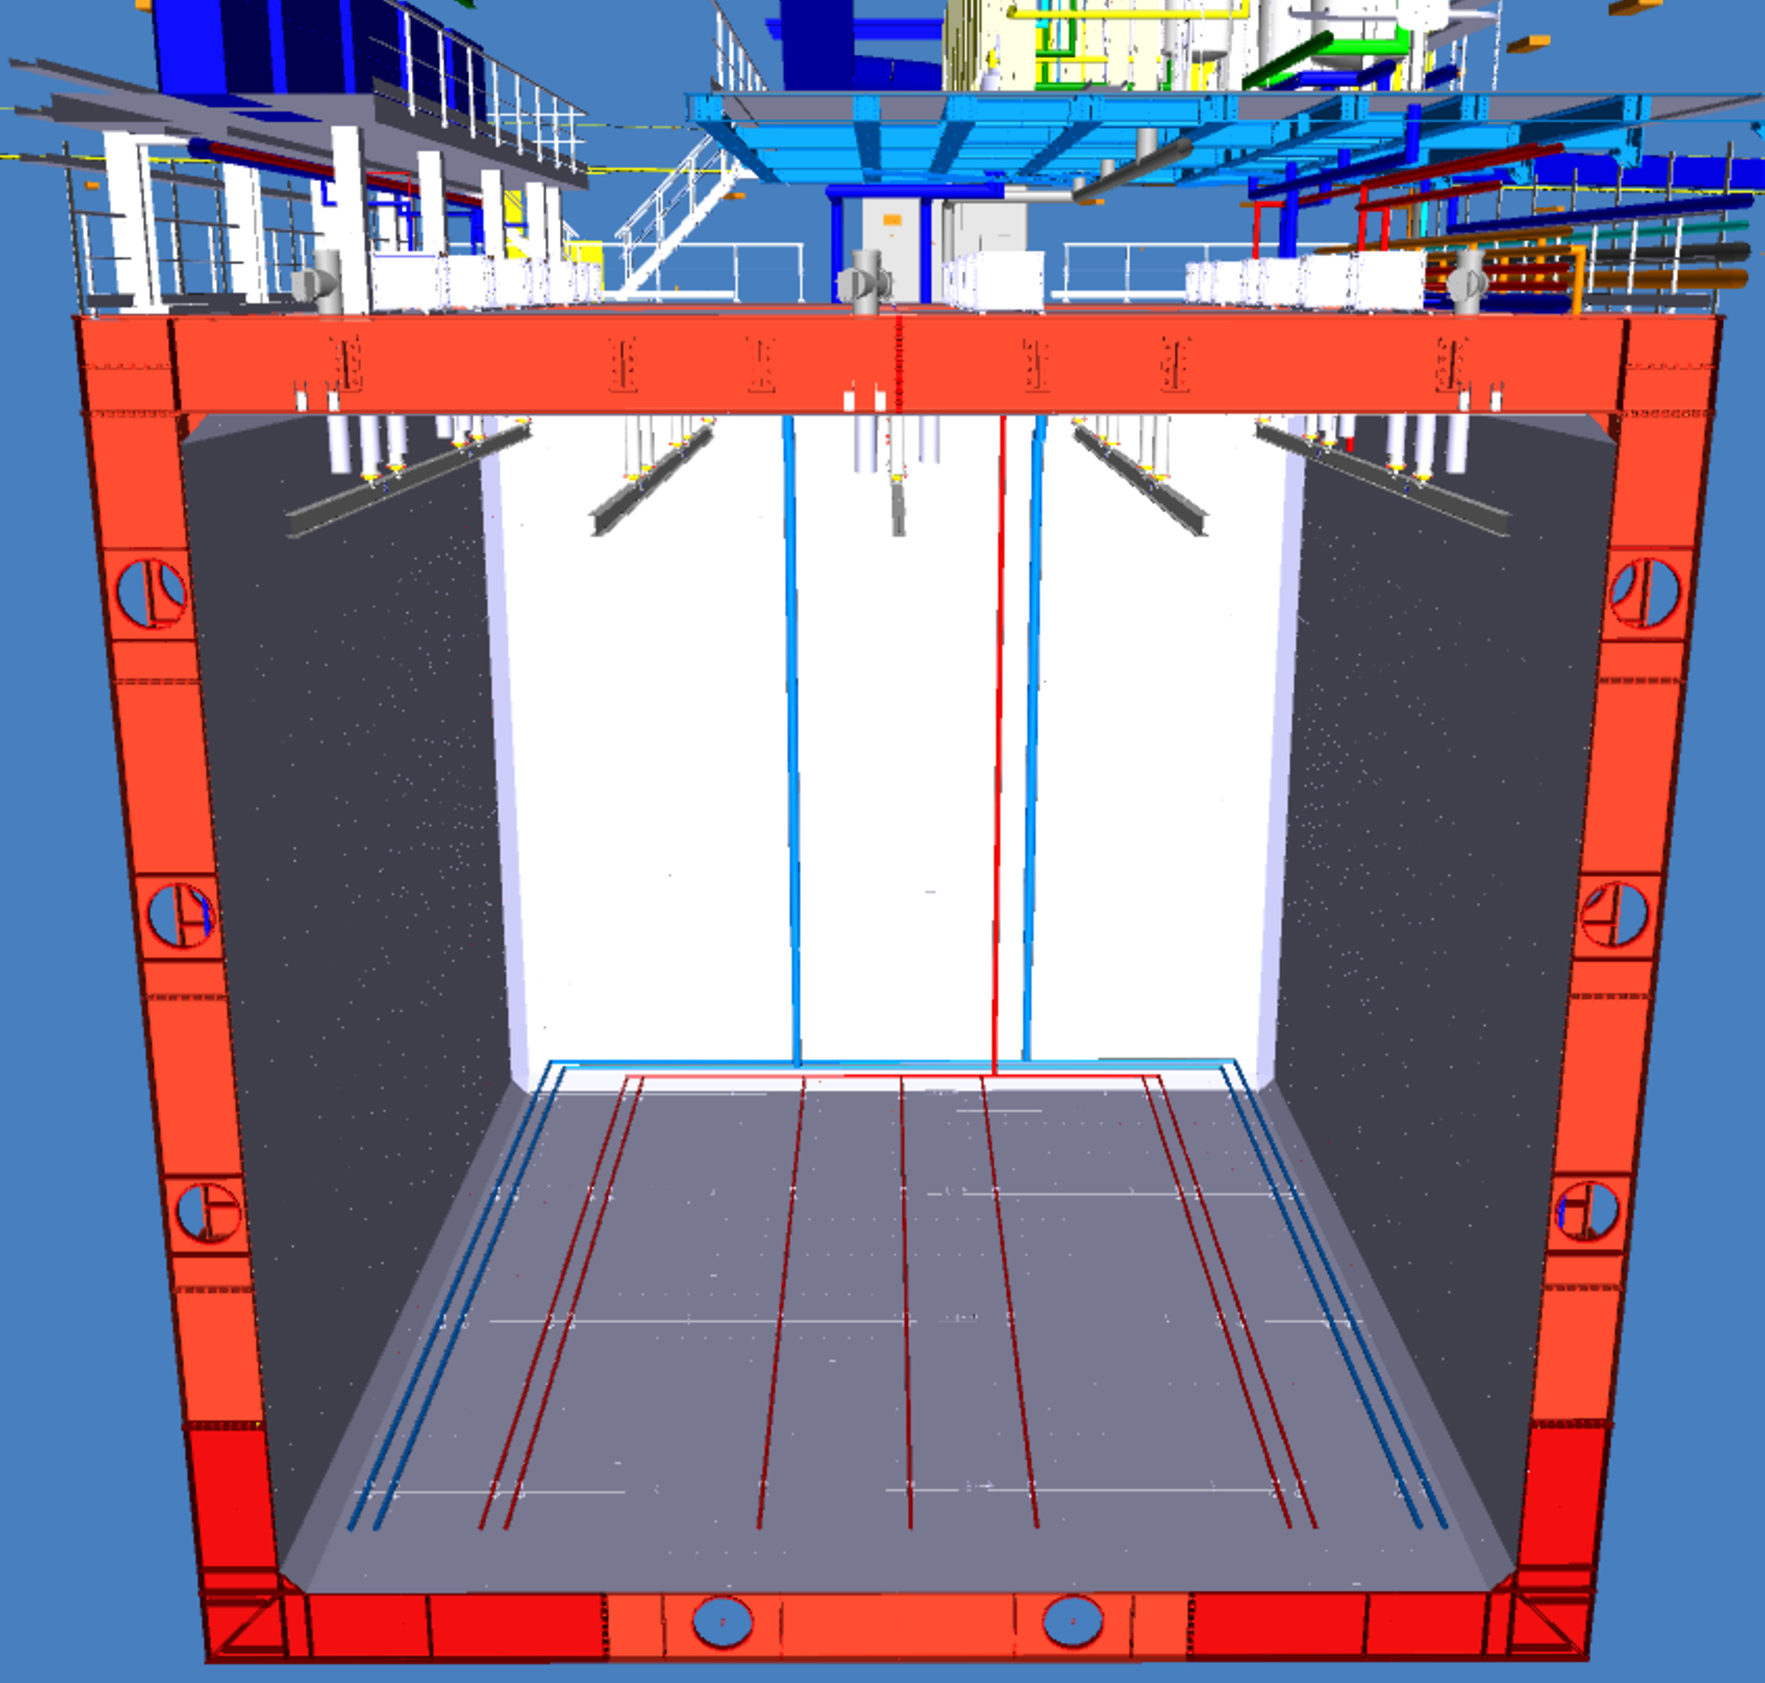
\includegraphics[width=.98\textwidth]{graphics/Internal-Piping-3D.pdf}
\end{dunefigure}

%\begin{dunefigure}[Drawing of the cryogenic %piping inside the cryostat %]{fig:internal-cryo-drawing}
%  {Drawing of the internal cryogenics.}
%\includegraphics[angle=90,width=.98\textwidth]{%graphics/Internal-pipes-HQ.pdf}
%\includegraphics[angle=90,height=.98\textheight%]{graphics/Internal-pipes-HQ.pdf}
%\end{dunefigure}
%\fixme{Please reduce size of Internal-pipes-HQ.pdf}


Other infrastructure inside the cryostat includes the cryostat false floor, the UV filtered lighting, and the battery-operated scissor lifts. 

The false floor requirements are not yet fully defined.  
It must support the load of the scissor lift used to work on the electronic cabling on the inside of the cryostat near the ceiling and allow the scissor lift to get close enough to the \dword{apa}s to work comfortably at the top. 
It  must be laid out so the panels can be removed in sections just before the equipment is installed. 
This is especially important for the \dword{apa}s where there is not enough room between the bottom of the \dword{apa}s and the floor to allow removal after installation. 

The cryostat lighting, using UV-filtered \dword{led} lamps, is expected to be fairly simple. Options for the lighting will be developed during the Ash River testing.
Floor-mounted lights with task lighting will be investigated. If needed, lighting can also be mounted to the \dword{dss} and removed as the detector is installed.

The plan is to use a commercially available battery-operated scissor lift with a SI{12}{m} reach. Tests at Ash River will verify the stability of the lift at height. If the lift is determined to be suitable, then the remaining issue to resolve is how to install and remove it from the cryostat. 
The commercially available scissor lifts are too wide to fit through the \dword{tco} near the floor where the center post protrudes above floor level.
Custom lifting equipment will be needed to insert the lifts into the cryostat. 
At the end of the installation process, dismantling the last lift may be necessary to remove it from the cryostat.

% clear the figure buffer before starting the next section
%\clearpage

%%%%%%%%%%%%%%%%%%%%%%%%%%%%
\subsection{Cleanroom Infrastructure}
\label{sec:fdsp-tc-infr-comm}

\begin{dunefigure}[Installation Cleanroom layout]{fig:install-cleanroom}
  {Two views of the installation cleanroom.  The top view shows the cleanroom in position in the north cavern. The location of the material airlock and the changing room are indicated. The lower image is a closer view showing the equipment in the cleanroom. The cryostat is shown in red.
  } 
%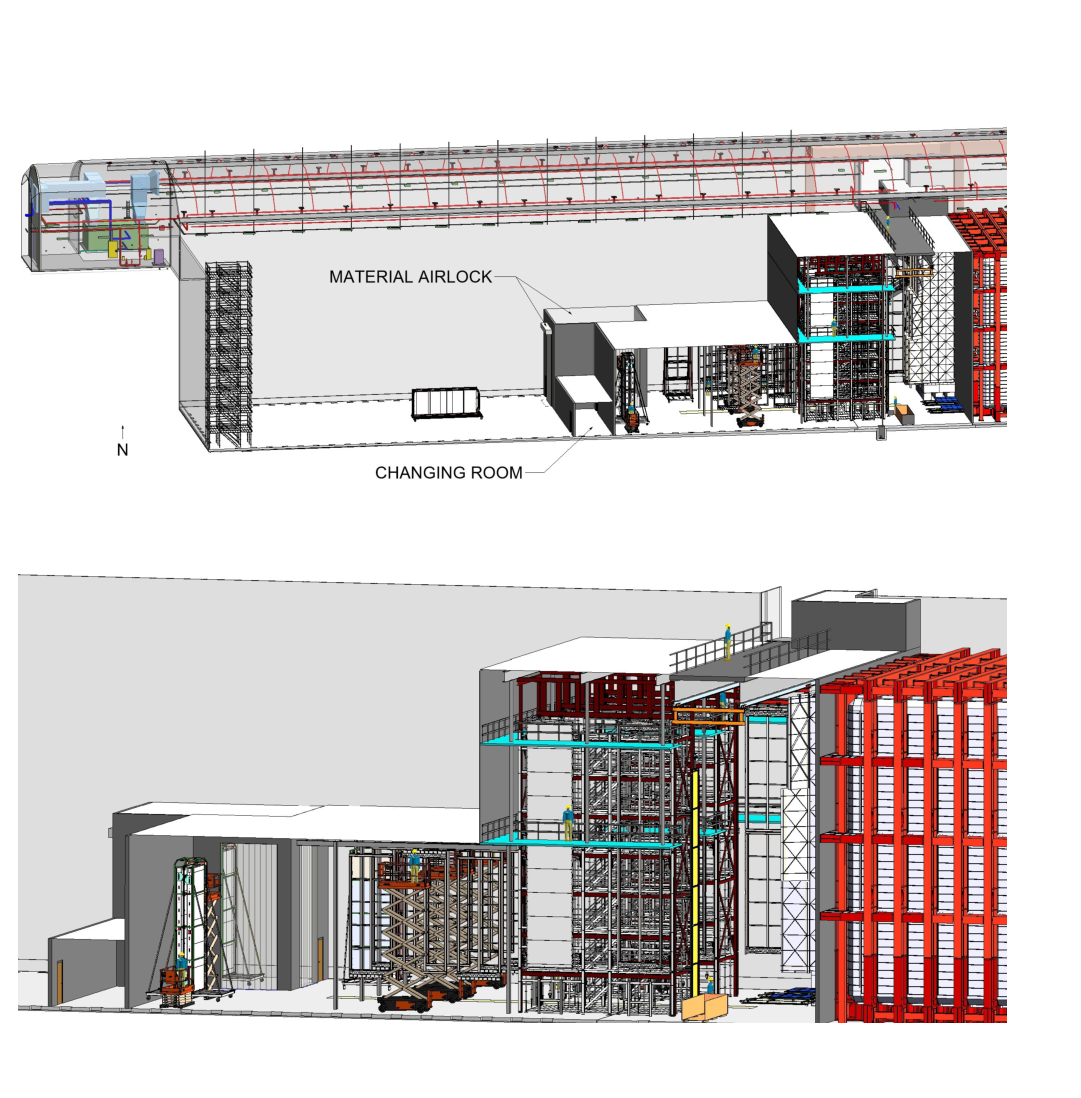
\includegraphics[width=1.0\textwidth]{graphics/install-cleanroom.pdf}
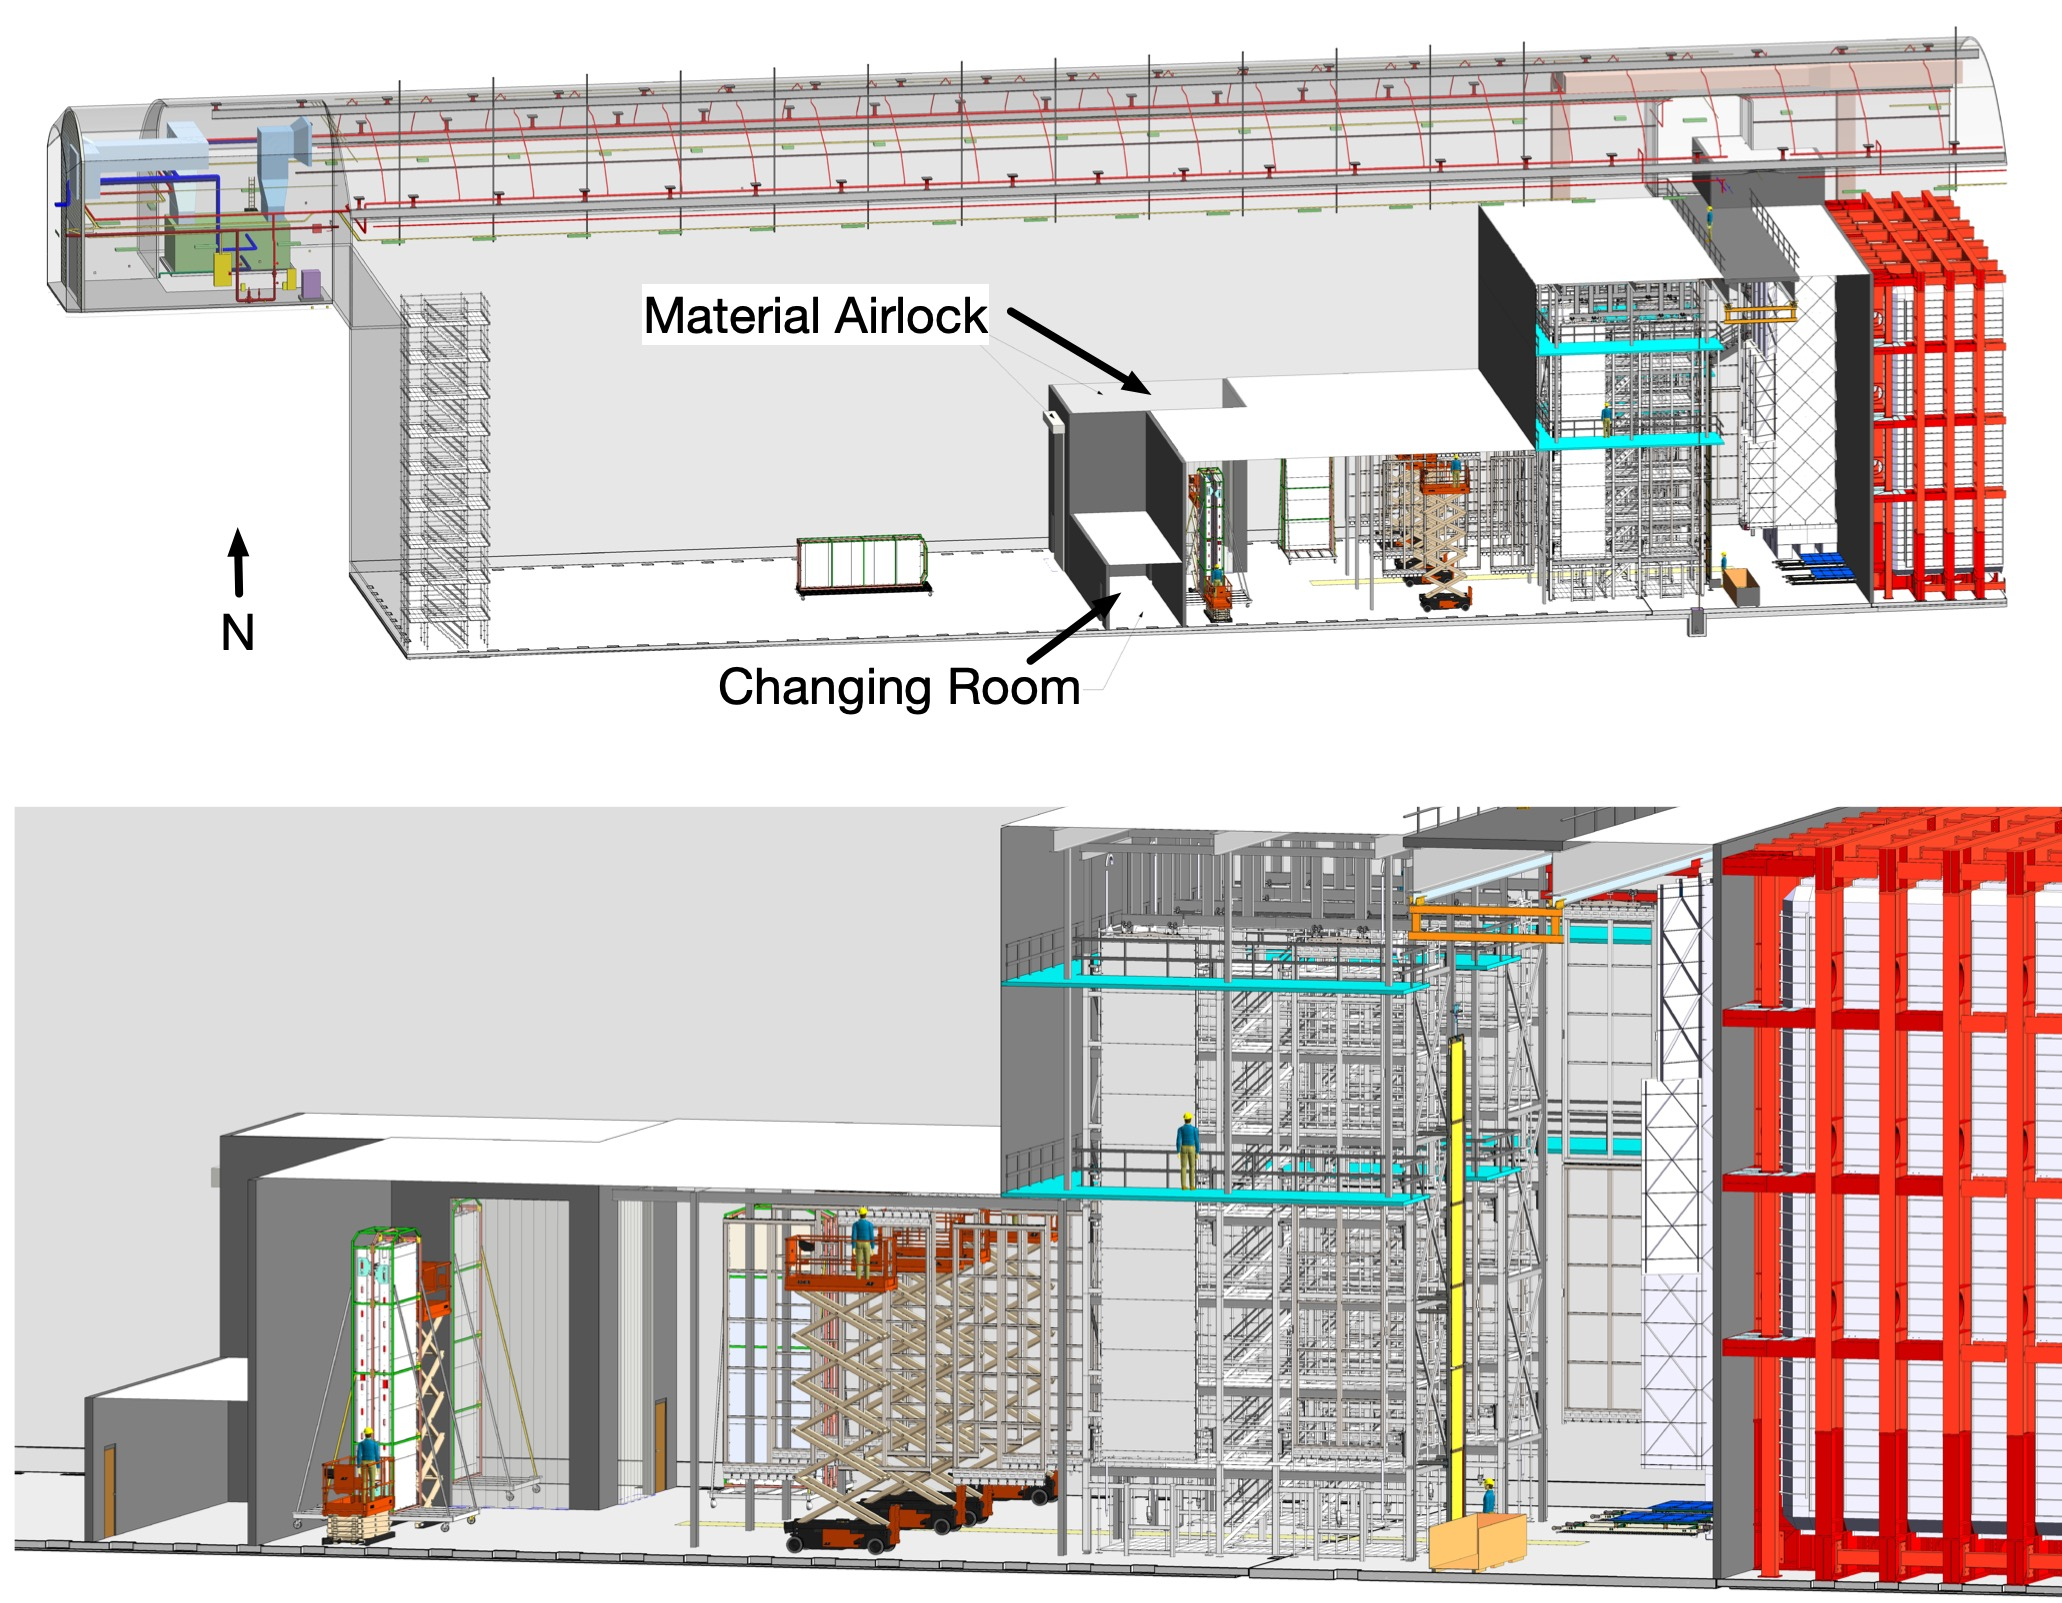
\includegraphics[width=1.0\textwidth]{graphics/install-cleanroom.jpg}
\end{dunefigure}

The cleanroom infrastructure consist of the cleanroom itself, the coldboxes and cryogenic plant for testing the assembled \dword{apa}, the assembly towers, rails and switchyard to allow the \dword{apa} to move inside the cleanroom, and the PD integration infrastructure. A combination of contractors and the lead worker and rigger teams will do the infrastructure work; they will also assist in detector assembly. 

The assembly of the detector sub-components into \SI{12}{m} tall full assemblies must be done underground directly outside the cryostat. 
The full assemblies are too large and fragile to be brought down the shaft, and the only place with enough vertical space to assemble them is in front of the cryostat itself. 
\dword{protodune} showed that it is critical to cryogenically test the completely assembled components immediately before installing them in the cryostat as this was the single step that found all the detector issues. 
The requirement that final assembly and testing be performed underground next to the cryostat implies that a suitable cleanroom be set up outside the cryostat. 
The cleanroom must meet the ISO-8 cleanroom standard to maintain the cleanliness of all the components entering the cryostat.  
Air will be filtered and then forced into the cryostat at the east end. The clean air will flow through the cryostat and out through the cleanroom and airlock. 
This will keep the inside of the cryostat at least at ISO-8.  
The airlock, cleanroom, and inside the cryostat will be outfitted with UV filtered lights to protect the photon detectors.

The dimensions of the cleanroom are determined by first planning the work performed inside. After the work flow is defined and the equipment needed has been sketched out the envelope of the work are can be established and the size of the cleanroom defined. Figure \ref{fig:install-cleanroom} illustrates  the conceptual design of the installation cleanroom. The top figure shows the cleanroom situated in the cavern next to the cryostat, the materials airlock and the changing room are on the west end. The bottom image is a closer view showing some of the equipment in the cleanroom. 



All the detector elements enter the cleanroom by passing through a materials airlock (Figure \ref{fig:install-cleanroom}). 
The material enter through large rollup doors that are sized to allow an \dword{apa} transport box (\SI{2.6}{m} by\SI{6.8}{m}) to enter in a vertical orientation. 
The airlock is \SI{7.5}{m} wide, \SI{5}{m} deep, and \SI{10}{m} tall while the rollup doors are \SI{3}{m} wide and \SI{7.5}{m} tall. 
It is expected the \dword{apa} box will be bolted to a custom pallet and moved with electric pallet jacks so door dimensions are sufficient. 
The changing room is 6 \si{m} wide and 7 \si{m} deep. 
The dimensions were chosen to allow 50 people to gown up for the cleanroom within a reasonable time. 
The requirements for work in an ISO-8 cleanroom are a cleanroom lab coat, clean shoes, and nets for hair and beards.  
This will be augmented with a clean hard hat and gloves for safety reasons. 

%The cleanroom proper can be as divided into three primary work areas: the integration area, the APA assembly and cabling area, and the HV assembly and cryogenic testing area. 

The cleanroom proper can be divided into several work areas as follows:
\begin{itemize}
\setlength\itemsep{1mm}
\setlength{\parsep}{1mm}
\setlength{\itemsep}{-5mm}
    \item Materials and Personnel airlocks,
    \item \dword{pd} integration area,
    \item Four \dword{apa} assembly lines where the lower rails are for wire tension measurements and the upper rails for APA  assembly and cabling,
    \item The switchyard area used to move the assembles APA in the cleanroom and into the cryostat,
    \item The \coldbox area where the APA are cold tested, and
    \item The HV assembly area.
\end{itemize}

\begin{comment}
The integration area at the west end of the cleanroom is where the \dword{pd} and \dword{ce}-\dword{femb} are integrated into the \dword{apa} and where the receiving quality assurance tests are performed. 
The activities are time consuming so three assembly lines are planned to keep up with the rate of installation in the cryostat. 
A fourth line is available for spare capacity and repair. 
The integration area measures \SI{19.5}{m} wide by \SI{21}{m} deep with a \SI{10}{m} ceiling, including the airlock area. 
A similar design is considered as what was used for the \dword{protodune} cleanroom as the height is similar. 
If needed the rail system inside the integration work area can be used to support the roof.
\end{comment}

The \dword{pd} integration area at the west end of the cleanroom is where the \dword{pd} are integrated into the \dword{apa} and where the initial receiving quality assurance tests are performed. 

Because the testing and assembly of the \dword{apa} into \SI{12}{m} tall doublets is time consuming the cleanroom has 4 assembly lines in order to keep up with the detector cold tests and installation. 
Three lines will be in continuous usage and the 4th for repairs or contingency. 
Each assembly line has a lower and upper set of rails fro moving the \dword{apa}.
The lower rails are where the wire tension is measured and the lower \dword{ce} \dword{femb} are installed. The \dword{pd} integration area and the lower rail section of the assembly lines measure \SI{19.5}{m} wide by \SI{21}{m} deep with a \SI{10}{m} ceiling, including the airlock area. 
A similar design is considered as what was used for the \dword{protodune} cleanroom as the height is similar. 
If needed the rail system inside the integration work area can be used to support the roof.
 
The \dword{apa} assembly and cabling area is where the top and bottom \dword{apa} are connected together to form a doublet and the \dword{ce} cables are inserted and connected to the \dword{femb}. 
This area has to be taller as the full \SI{12}{m} tall \dword{apa} doublets must be accommodated. 
The ceiling in this area is \SI{17.8}{m} placing the ceiling at the same level as the bridge and the roof of the cryostat. 
A \SI{9}{m} by \SI{19.5}{m} area is sufficient to house the two large assembly towers needed to support the assembly lines. Above the towers I-beams running north-south or transverse to the neutrino beam are needed to support work platforms which allow access to both faces of the \dword{apa}s these beams can be used to support the cleanroom roof which can be a light weight frame with a fire retardant fabric attached. 
The outer towers steel structure provides a strong surface to attach a polymer sheet serving as the vertical wall connecting the \SI{17.8}{m} region to the \SI{10}{m} tall area.

The switchyard area is the region under the north-south bridge where a bridge crane is mounted and is used to move the \dword{apa} from the assembly lines to the \coldbox{}es and into the cryostat. The \coldbox{}es and the HV assembly area are between the bridge and the cryostat.


The cleanroom is as wide as the cavern excavation. The side walls of the cleanroom will be consrtucted by hanging reinforced fire retardant plastic sheets against the wall. This will result in a low cost construction that is easy to install.


\begin{dunefigure}[Installation Integration Rail System]{fig:install-integrate-rail}
  {Two pairs of rails are used to prepare the \dword{apa} for assembly. Each rail will hold three \dword{apa}. Here the wire tension measurements are performed and the \dword{ce} \dword{femb} are installed on the lower \dword{apa}. The lower \dword{ce} are easily reachable from the floor in this arrangement. This view is from the assembly towers looking west along the assembly lines.}
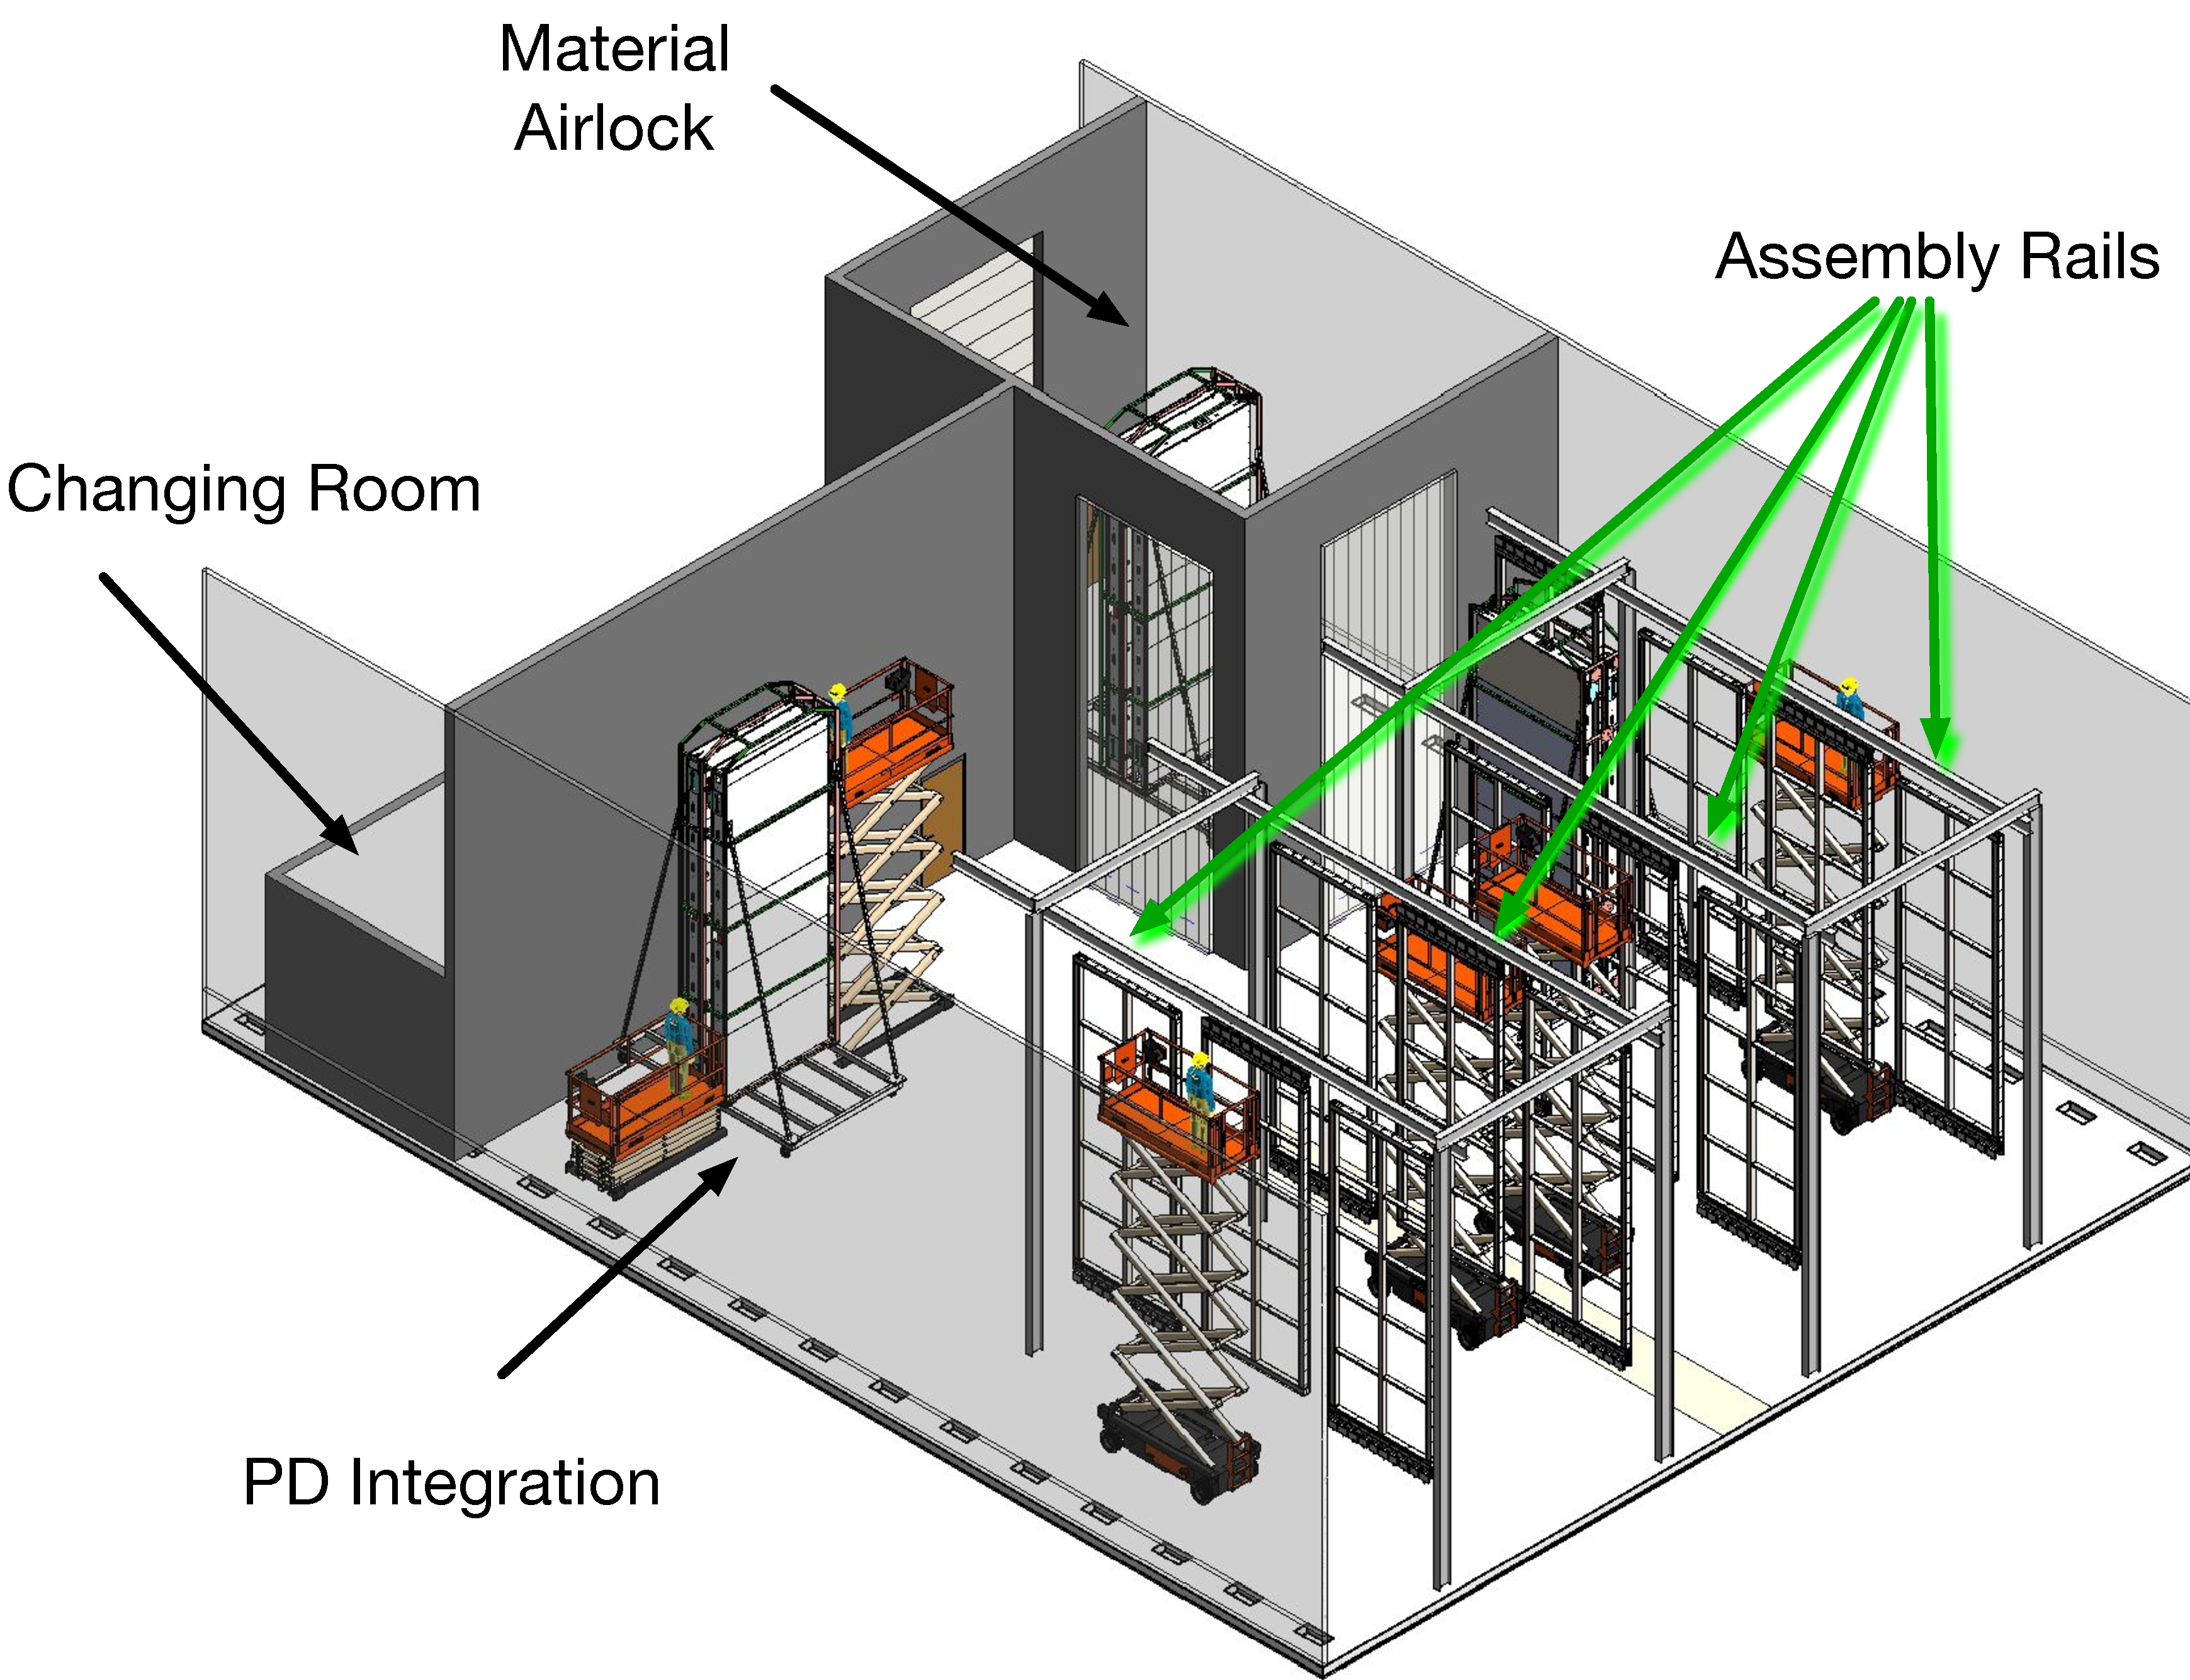
\includegraphics[width=.5\textwidth]{graphics/install-integrate-rail.pdf}
\end{dunefigure}

Given the substantial size and the significant occupancy, the cleanroom will have electrical outlets, UV filtered lighting, and fire protection.

Equipment in the integration work area will consist of a station for integrating the photon detectors into the \dword{apa} and two pairs of rails for preparing the \dword{apa} for assembly and several scissor lifts for working around the \dword{apa}. 
The area adjacent to the materials airlock is reserved for integration the \dword{pd} into the \dword{apa}. 
The \dword{apa} transport box will be positioned between two fixed lifts. 
The lifts are raised until the photon detector paddles can easily be inserted into the side of the \dword{apa}.
Figure \ref{fig:install-integrate-rail} illustrates the rail setup in the integration work area. 
The \dword{apa} are removed from the transport box and mounted to the rails at the far end. 
They then move along the rails using simple trolleys running on the I-beams. 
The rails are long enough to hold three \dword{apa} at a time. 
This setup is conceptual and engineering design of the rail supports has not yet started. 
Cross bracing of the vertical posts will be added during the design stage. 

\begin{dunefigure}[APA cabling tower]{fig:install-assembly-tower}
  {The \dword{apa} assembly and cabling tower is shown in three views: isomtetric, north face and south face (left, center, and right images respectively). 
  The tower is designed to be two \dword{apa} wide so work on two \dword{apa} side by side. Both the north and south face are equipped with assembly rails so a single tower supports two assembly lines.
  The work decks allow access to the \dword{apa} from multiple levels.
  The two reels of cable for the electronics are shown. }
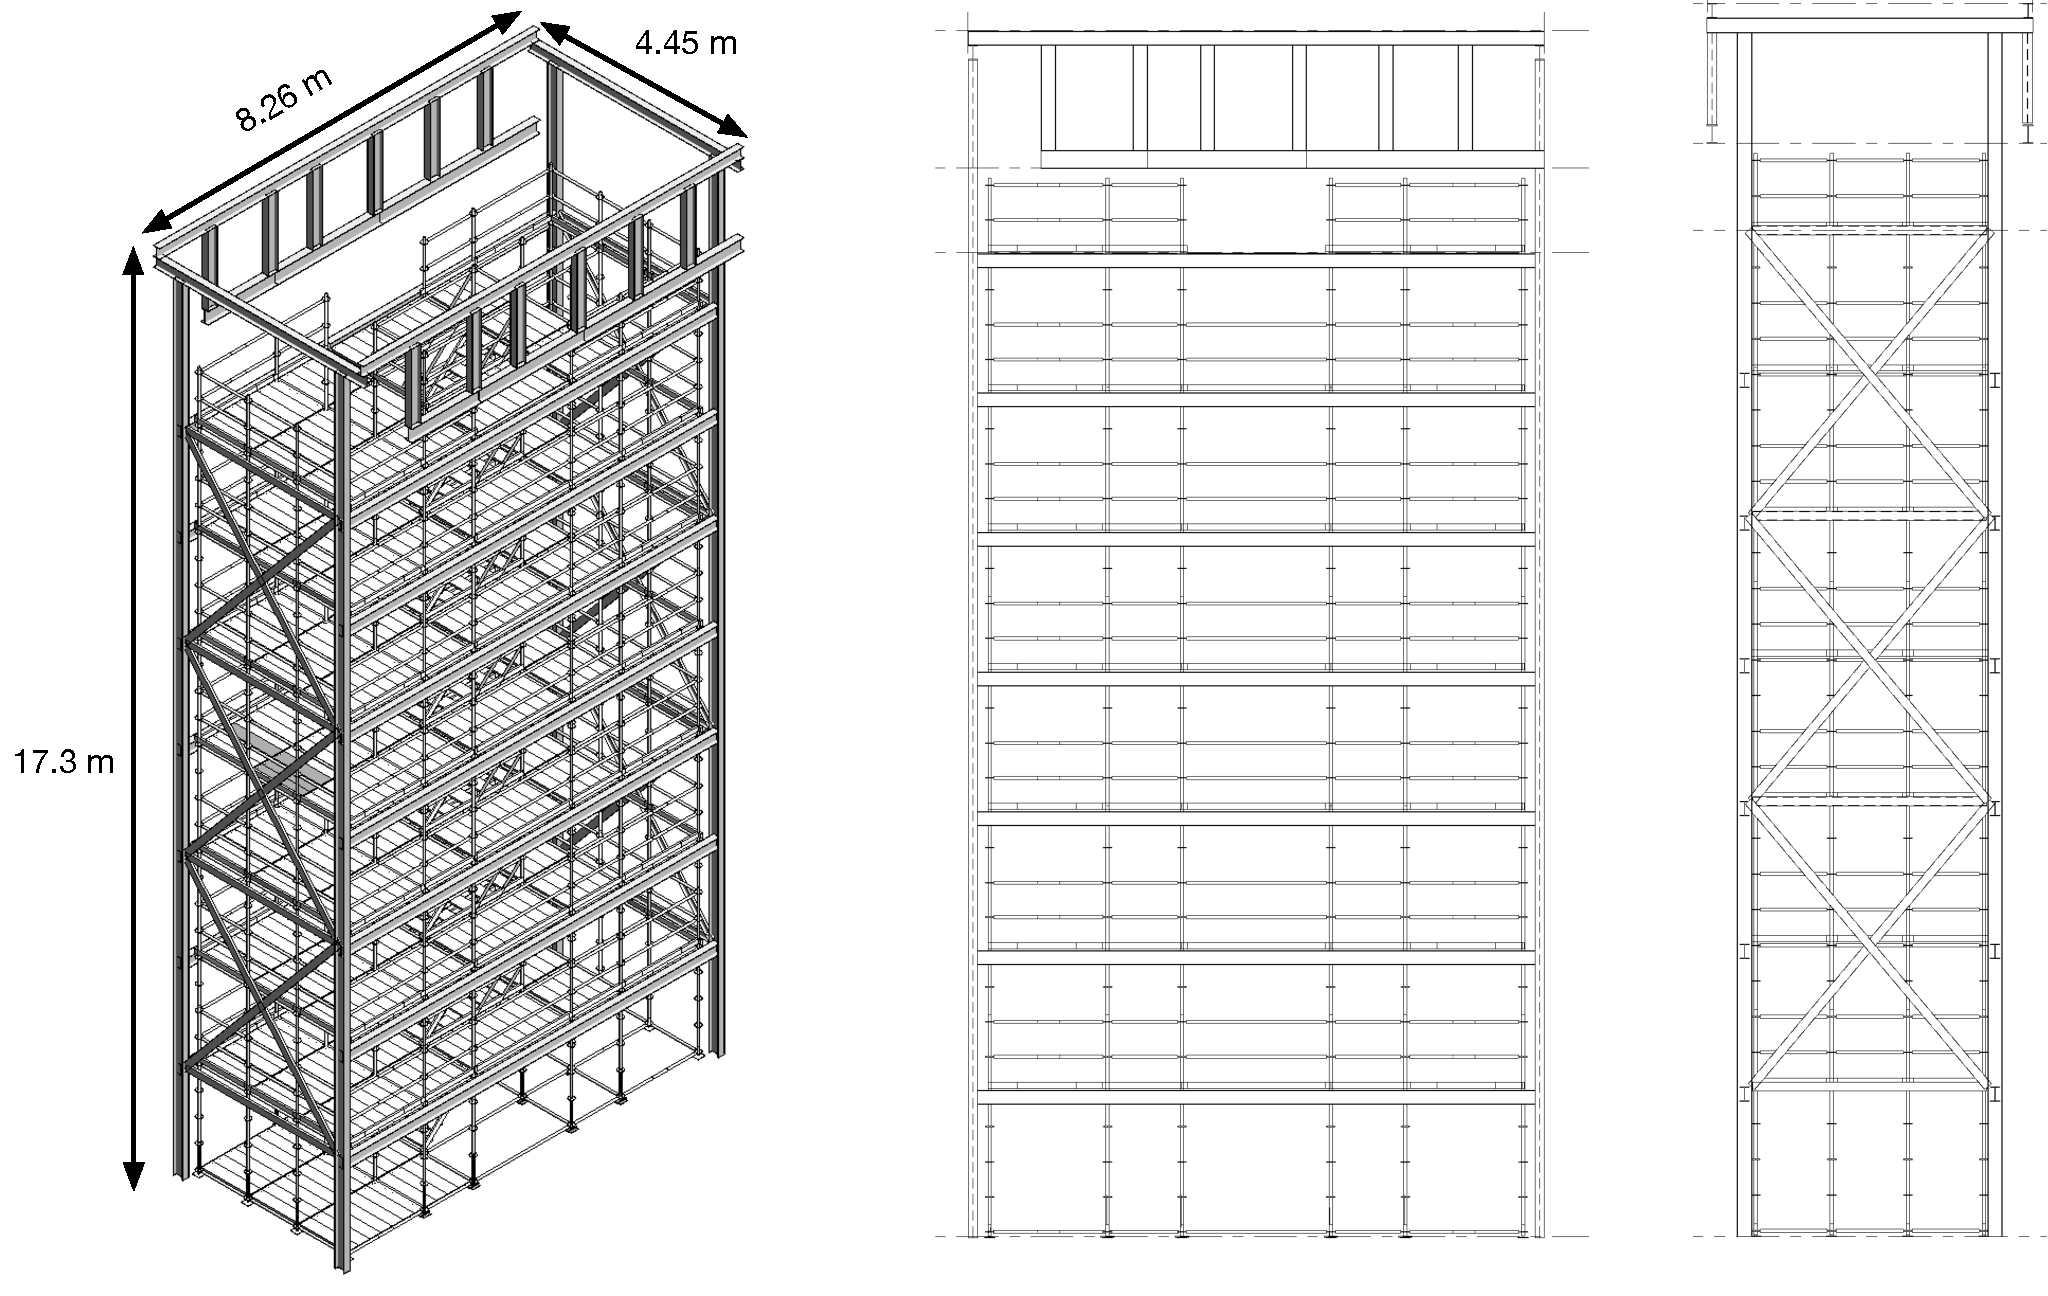
\includegraphics[width=.95\textwidth]{graphics/install-assembly-tower.pdf}
\end{dunefigure}


In the \SI{17}{m} tall  \dword{apa} assembly and cabling area of the cleanroom two large work towers (shown in Figure \ref{fig:install-assembly-tower}) support the four assembly lines. 
These \dword{apa} assembly and cabling towers are where the upper and lower \dword{apa} are assembled together, the \dword{ce} cable is inserted through the \dword{apa} doublet, the cables are connected and arranged for transport, and the electronics are warm tests. 
These towers are designed to be wide enough to hold two \dword{apa} side by side with enough space between to walk through or work. 
The tower is seven stories tall with work areas at each landing.
Rails at mid-height and at the top of the towers are used to move the \dword{apa} to the different locations along the tower. 
The \dword{apa} assembly cabling tower also provides support for the the \dword{apa} assembly fixture provided by the \dword{apa} consortia. 
The \dword{apa} assembly fixture is the tooling needed to hold the upper and lower \dword{apa} during assembly and to bring the two modules together so they can be connected. 
The  tower is conceived as a steel outer frame that supports the \dword{apa}s and the rails. Inside the steel frame is a standard scaffolding for people to use as a work platform. 
The scaffolding allows workers to assess the \dword{apa} at different heights. 
The scaffolding is wide enough for people to be working on both sides simultaneously and for a stairway in the middle that meets OSHA standards. 
North-south beams will be places on top of the tower to support the cleanroom roof and the work platforms shown in Figure \ref{fig:install-workdeck}.
The image shown in Figure \ref{fig:install-assembly-tower} is a modified model based on a single wide \dword{apa} tower which has passed all safety reviews and has already been constructed. 
This double-wide tower will need to be re-engineered to insure that all the beam dimensions and bracing are appropriate for the larger spans and loads. 
It will then go back through the full safety review and the initial prototype of the tower wil be fabricated for use at Ash River. 
The size and the layout of the top level of the tower will be optimized based on input from the Ash River tests. 


\begin{dunefigure}[Cleanroom platforms and material transport system]{fig:install-workdeck}
  {Work platforms, transport rails and switchyard in the installation cleanroom. This image shows a single wide tower but the final towers will accomodate 2 APA.}
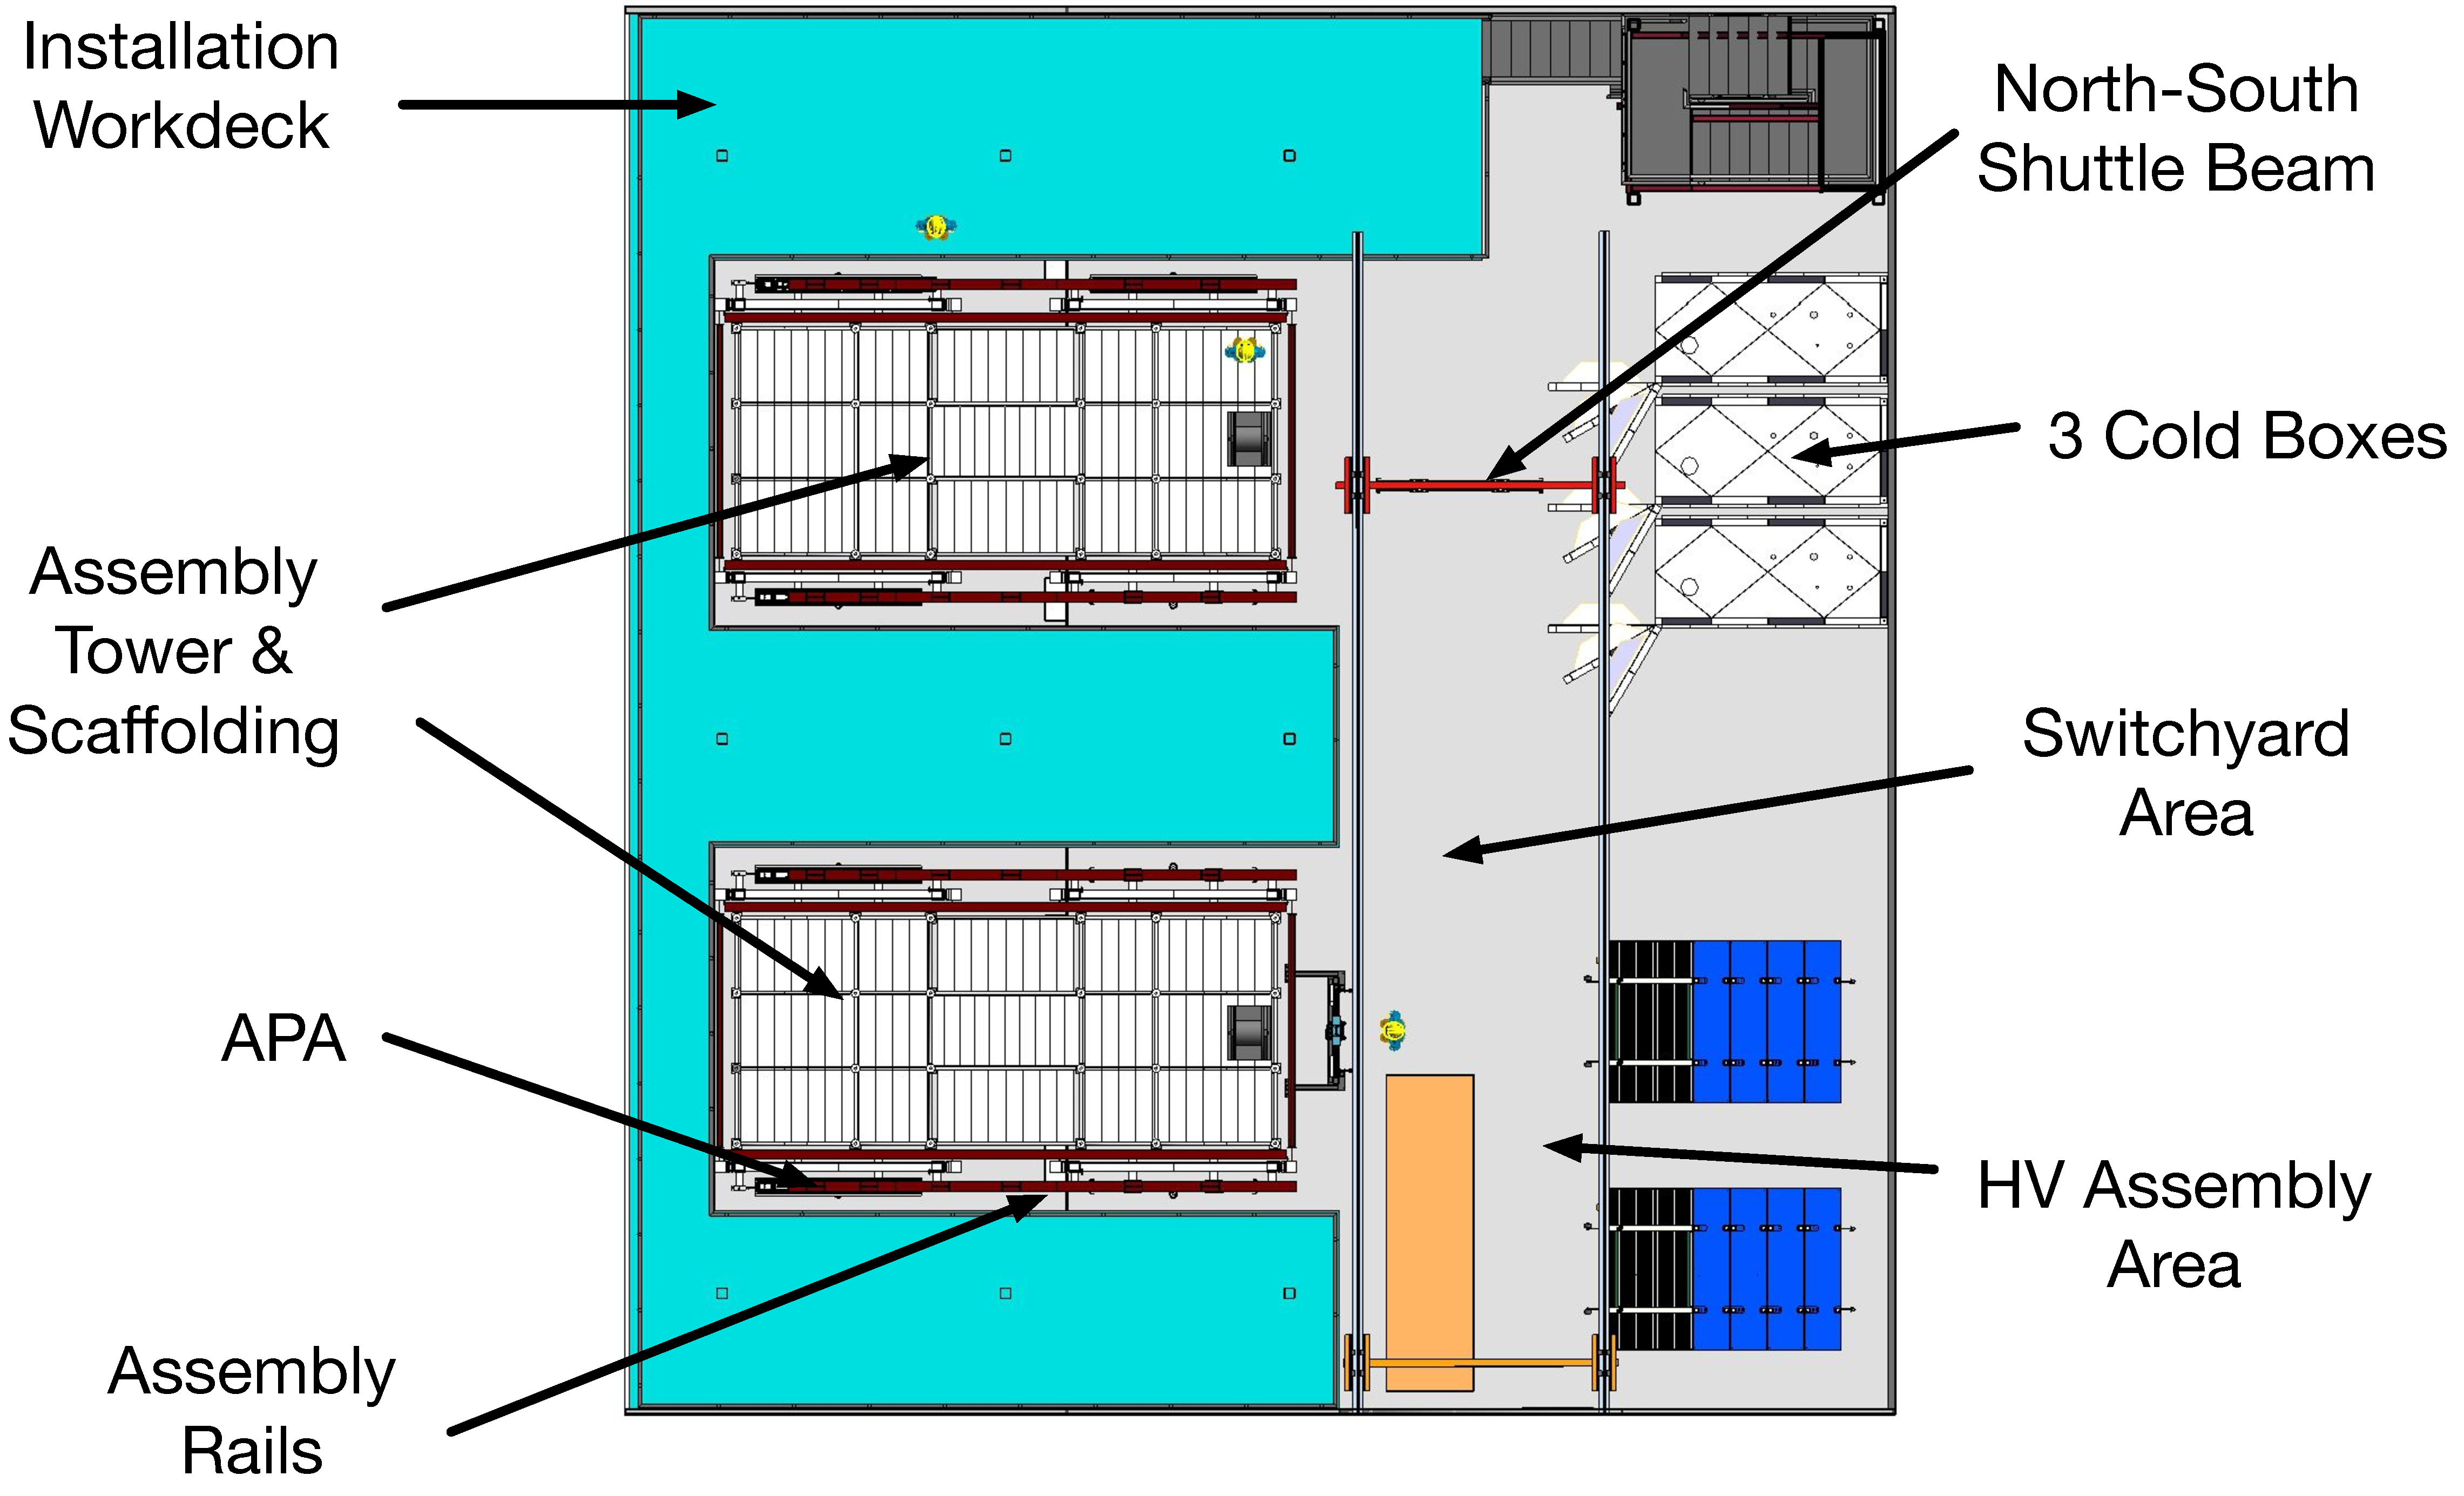
\includegraphics[width=.5\textwidth]{install-workdeck}
\end{dunefigure}

Because the cables can only be inserted through the \dword{apa} frames after the \dword{apa} doublet has been assembled a large amount of work must be performed at the \SI{15}{m} height of the TCO beam. 
The \dword{apa} assembly and testing towers described above provide a solid safe work platform for one side of the \dword{apa}s.
However access to both sides is required to connect the cables to the \dword{femb} and to properly bundle the cable into the cable trays in a way that allows the cables to easily be installed in the cryostat. 
Given the large number of person-hours needed for work at height all measures should be take to ensure that this work is as safe as possible. For this reason a series of stable fixed work platforms will be constructed as shown in Figure \ref{fig:install-workdeck}.
By running north-south beams from the cavern walls across the assembly towers strong rigid support points are provided. 
Vertical posts down from these beams can then support fixed work platforms as needed. Access to the work platforms is provided by drawbridge like retractable walkways between the middle of the assembly tower and the platform. 
A second means of egress is also provided by a connection from the fixed platforms to the permanent stairs. 

\fixme{need to get the height of the TCO beam from the cavern floor.}


Once the \dword{apa} doublet is assembled it can be moved onto the switchyard under the bridge. 
This switchyard is illustrated schematically in Figure \ref{fig:install-workdeck} is essentially a bridge crane running under the cavern north-south bridge. 
Several bridge beams driven by electric trolleys  move on the runway beams of the crane.  
A rail at the bottom of the crane mates up to the fixed beams  from the assembly lines, the cold boxes, the TCO beams and the HV assembly area.
By aligning the bridge beams with a set of fixed beams supported from the cleanroom roof, the \dword{apa} and \dword{cpa} can be transferred from the fixed beams to the bridge crane and moved to different locations in the cleanroom. 
Figure~\ref{fig:install-workdeck} shows a the 4 fixed beams on the 4 assembly towers, the 3 fixed beams for the cold boxes and the two fixes beams for the TCO. 
The \SI{12}{m} tall \dword{cpa} panels will be assembled directly under the bridge crane and transferred directly form the assembly fixture to the switchyard crane.

%%%%%%%%%%%%%%%%%%%%%%%%%%%%
\subsection{Cryogenics and \coldbox{}es}
\label{sec:fdsp-tc-infr-cryo}



After an \dword{apa} pair is fully assembled and cabled but before installation in the detector cryostat, it is thermally cycled in a tall narrow test cryostat, called a \coldbox{}, shown in Figure~\ref{fig:install-coldbox}). 
To test \dword{apa}s at a rate necessary to keep up with the installation plan, we will use three identical \coldbox{}es in the cleanroom. 
The \coldbox{}es require a dedicated cryogenics system that cools them  close to \dword{lar} temperature. 


A \coldbox has external dimensions of 14.0 \si{m} by 3.2 \si{m} by 1.3 \si{m} (H $\times$ L $\times$ W). With three layers of 100 \si{mm} thick foam insulation,  
the internal dimensions are 13.4 \si{m} by 2.6 \si{m} by 0.7 \si{m}. A rail section similar to those used elsewhere in the cleanroom will be mounted inside each \coldbox to allow the cleanroom switchyard and trolleys to push an  \dword{apa}  into a \coldbox. The \coldbox{}es will be light tight when closed to support \dword{pd} testing. A support base under the \coldbox{}es will adjust the height to mate with the cleanroom switchyard.

 
The \coldbox electronics \fdth{}s  will be  similar to what is used on the top of the \dword{dune} cryostat, except that short cables will be run from the \dword{wec}  to a patch panel inside the \coldbox. This will allow the cable on the \dword{apa} to connect directly to the test readout without having to remove any cabling. The \coldbox  design is nearly the same as the successful \dword{pdsp} \coldbox. The outer shell is similarly constructed of a stainless steel plate with reinforcing ribs welded on. The height is of course doubled, and a hinged door is planned. Unbolting the door and lifting it off the \dword{pdsp} \coldbox required significant effort, and lacking full crane coverage in this case, doors that can be opened and closed using a scissor lift are necessary. The \dword{dune} \coldbox{}es will collectively need about 11 \si{T} of stainless steel, according to initial estimates. The \coldbox{}es may be assembled in place because the finished boxes are too big to fit down the Ross Shaft. As the design continues it will be investigate if the coxes can be assembled in pieces that can be brought underground separately and assembles. The \coldbox base will be on Hilman rollers, so the boxes can be moved under the bridge after detector installation  to allow installation of the cryogenic circulation pumps.




\begin{dunefigure}[Installation \coldbox]{fig:install-coldbox}
  {\coldbox{}es used to thermally cycle the fully assembled APA pairs. }
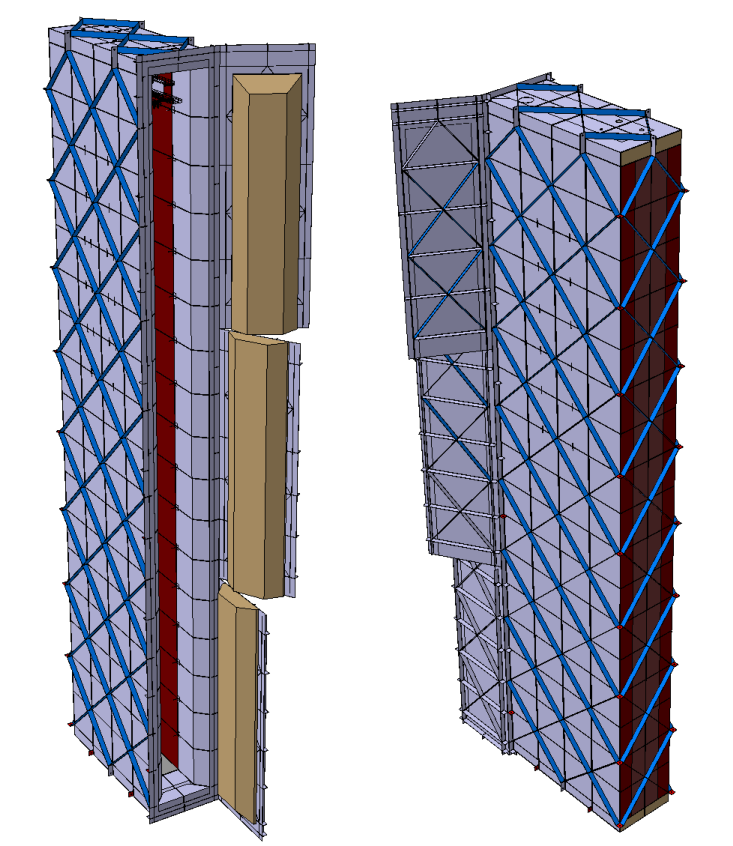
\includegraphics[width=.5\textwidth]{graphics/install-coldbox.pdf}
\end{dunefigure}


%{Cold Boxes Cryogenics}
\label{sec:fdsp-tc-cryocoldbox}

%The cryogenics supporting the \coldbox{}es underground must ensure reliable and safe operation of the system used to test the \dwords{apa} that will be installed inside the cryostats. The main functional requirements of the system are
The  \coldbox{}es will be used to test the \dword{apa}s underground prior to installation. % in the cryostat. 
The cryogenics supporting the \coldbox{}es  must ensure their reliable and safe operation; to that end, it must
\begin{itemize}
\setlength\itemsep{1mm}
\setlength{\parsep}{1mm}
\setlength{\itemsep}{-5mm}
\item support three \coldbox{}es operating in parallel: %for testing dual \dword{apa}s: 
one in \cooldown mode, two either in steady-state or warm-up modes.
\item allow personnel in the cleanroom during all phases of the purge, \cooldown, operation, and warm-up modes. 
\item test the detector modules at near \dword{lar} temperature.
\item operate 24 hours a day, seven days a week for 10 years.
\item allow remote operations.
\item be located in the vicinity of the \dword{tco}. Space is available on top of the cryogenic mezzanine on the roof of the cryostat.
\end{itemize}

It must operate in the following modes: %fulfill the following modes of operations:

\begin{itemize}
\setlength\itemsep{1mm}
\setlength{\parsep}{1mm}
\setlength{\itemsep}{-5mm}
\item \textbf{purge}: During this mode, air is removed from the system (\coldbox and cryogenic system) and replaced with dry nitrogen. The concentration of moisture is monitored, and when it no longer decreases, the \cooldown can commence.
\item \textbf{\cooldown}: Cold nitrogen is introduced into the system to cool the inside of the \coldbox and the \dword{apa} inside it. %it down and to cool down the detector contained inside the coldbox. 
This should take 24 hours, during which time the temperature decreases from room temperature to about \SI{90}{K}. 
\item \textbf{steady-state operations}: After reaching %the nominal temperature of 
approximately \SI{90}{K}, %the value is maintained for 48 hours, during which 
the detector is turned on and fully tested. % at cold. 
This takes about 48 hours.
\item \textbf{warm-up}: After completing the test, the system is %slowly 
warmed up to room temperature over a period of 24 hours. %This should take 24 hours, during which the temperature goes from approximately \SI{90}{K} to room temperature.
\end{itemize}

\begin{dunetable}
[\Coldbox  cryogenics system parameters] %for specifications]
{lc}
{tab:table-cryo-coldboxes}
{Table of parameters for the \coldbox cryogenics system.}
Parameter & Value 
\\ \toprowrule
Dual \dword{apa} thermal mass &  1,600 kg\\ \colhline
Temperature uniformity & $+60$ K / $-0$ K \\ \colhline
Electronics load & 300 W \\ \colhline
\Coldbox insulation thickness &  0.3 m \\ \colhline
Target \cooldown temperature &  \SI{90}{K} \\ \colhline
Target \cooldown duration &  24 hr \\ \colhline
Target steady-state duration &  48 hr \\ \colhline
Target warm-up duration &  24 hr \\ \colhline
Maximum cooling power  &  \SI{13}{kW}  \\ \colhline 
Maximum liquid nitrogen consumption  &  \SI{300}{l/hr}  \\ \colhline 
\end{dunetable}

The evaporation of liquid nitrogen provides the cooling power for the system. Warm nitrogen and a heater provide the heating power. At peak consumption, the expected maximum heat load is \SI{8.5}{kW}. Assuming a 50\% margin on the refrigeration load, the cryogenics system requires \SI{13}{kW} of net cooling power at peak consumption, which equals about \SI{300}{l/hr} of evaporating liquid nitrogen.

Two layouts are currently under consideration: (1) a closed loop with mechanical refrigeration, in which liquid nitrogen is generated {\it in situ}, circulated, and the spent nitrogen recondensed before being put back into the system; and (2) open loop, in which liquid nitrogen is transported underground by means of portable dewars, circulated, and the spent nitrogen vented away. For the closed loop, we would need a mechanical refrigeration capable of supplying \SI{13}{kW} of cooling. For the open loop, it is possible to use a \SI{2000}{l} dewar, which is commercially available and transportable up and down the Ross Shaft inside the cage. To supply the required amount of nitrogen, four trips per day are needed.

The current versions of the closed loop and open loop systems are presented in Figures~\ref{fig:mechanical-refrigeration} and~\ref{fig:LN2}, respectively. % . The current version of the open loop system is presented in Figure~\ref{fig:LN2}.

\begin{dunefigure}[\Coldbox cryogenics support system based on mechanical refrigeration ]{fig:mechanical-refrigeration}
  {Layout of the cryogenics supporting the \dword{apa} test facility with mechanical refrigeration (closed loop).}
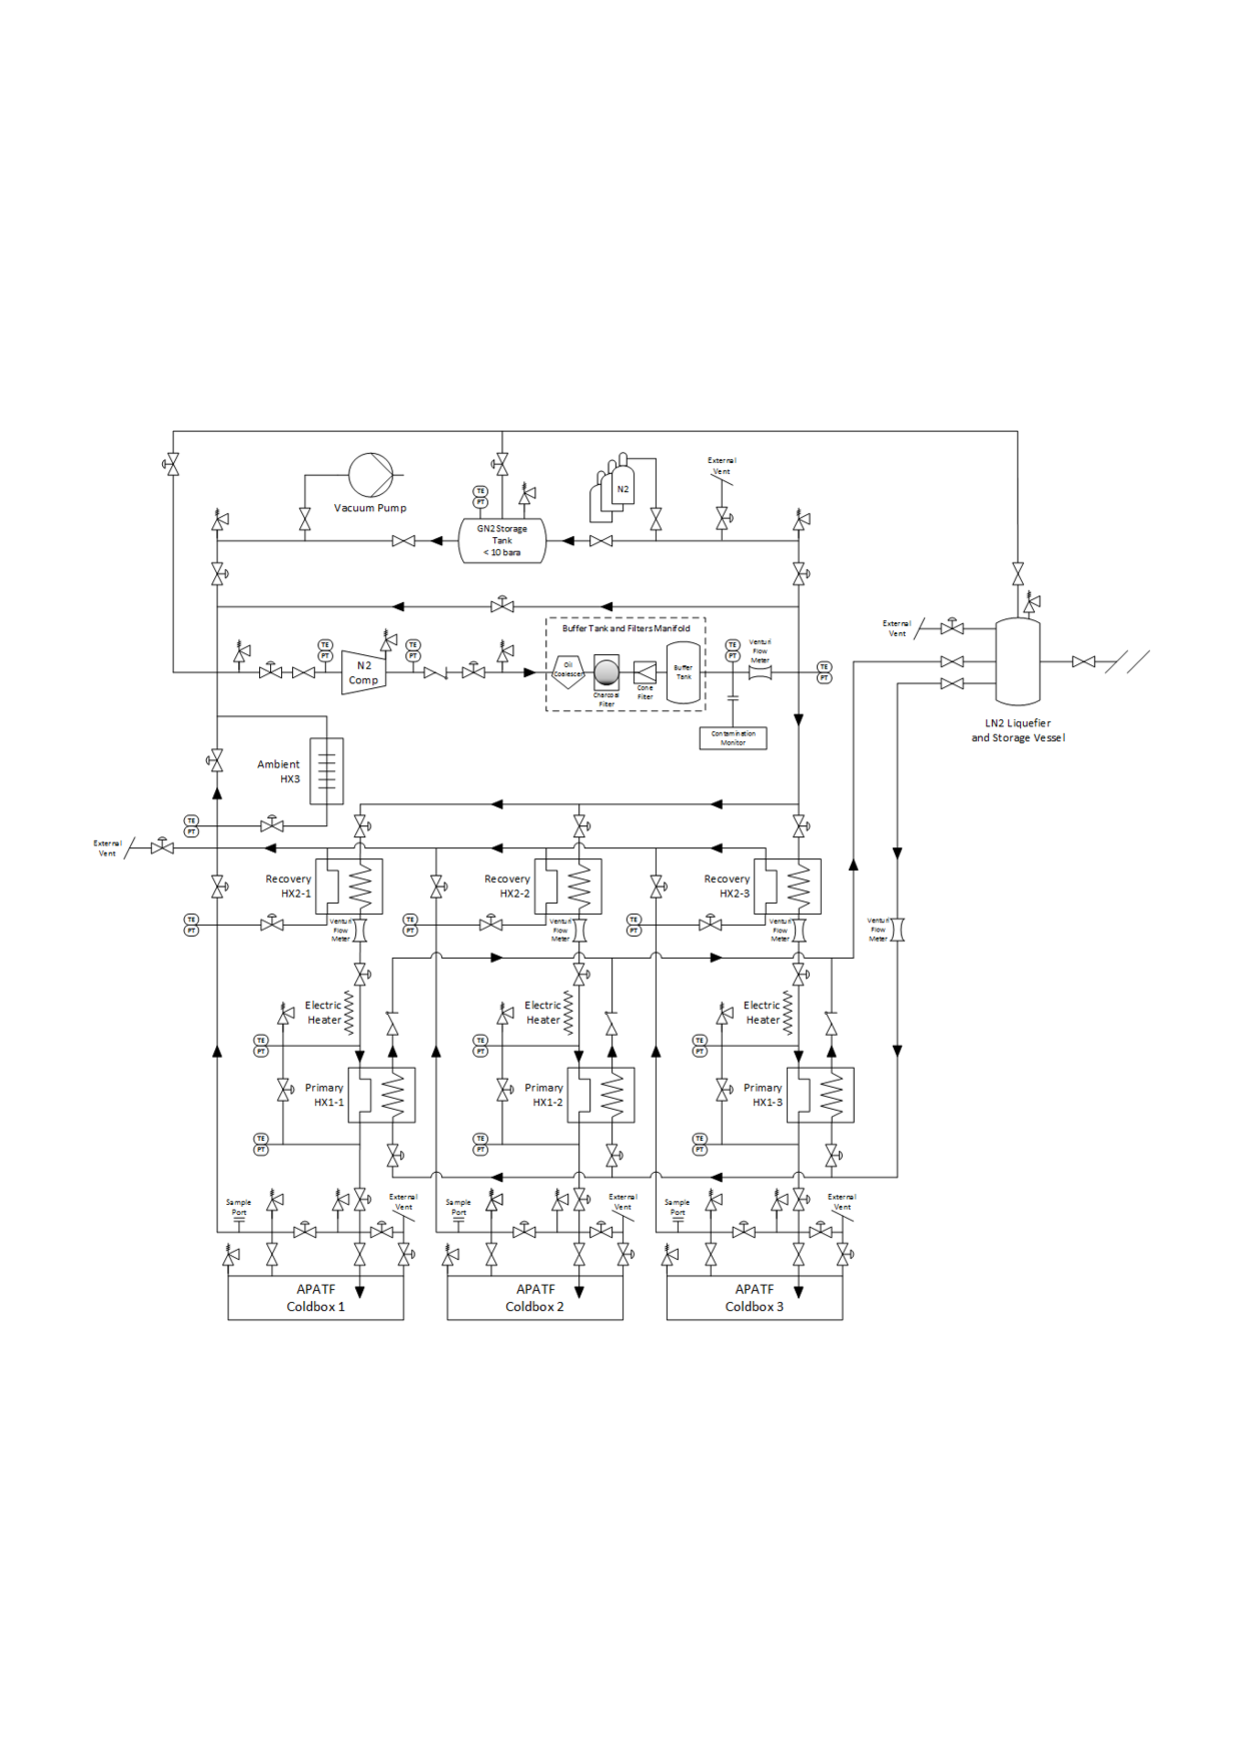
\includegraphics[width=.98\textwidth]{graphics/Cryo-cold-box-mechanical.pdf}
\end{dunefigure}

\begin{dunefigure}[\Coldbox cryogenics support system based on LN2 ]{fig:LN2}
  {Layout of the cryogenics supporting the \dword{apa} test facility with open loop refrigeration (open loop).}
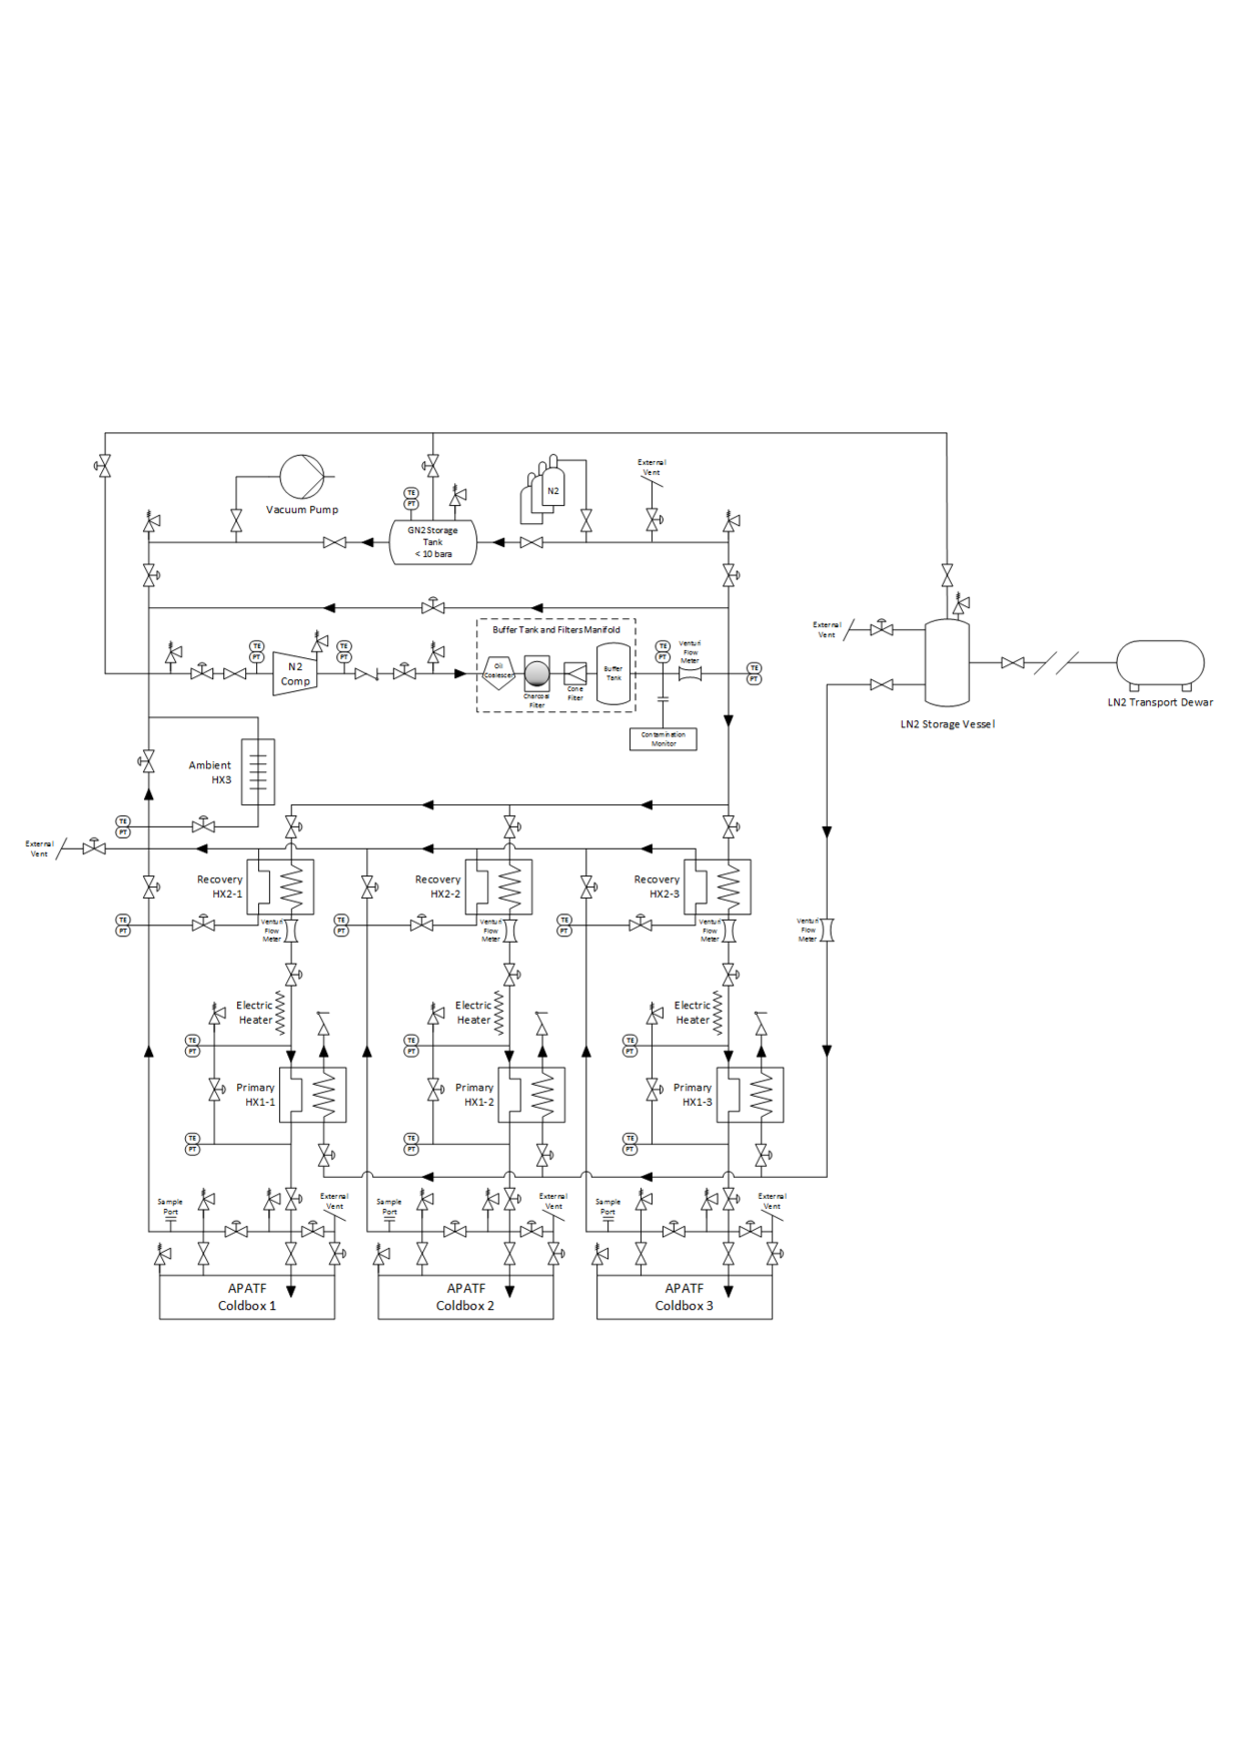
\includegraphics[width=.98\textwidth]{graphics/Cryo-cold-box-LN2.pdf}
\end{dunefigure}



%%%%%%%%%

% clear the figure buffer before starting the next section
%\clearpage

%%%%%%%%%%%%%%%%%%%%%%%%%%%%
\subsection{Prototyping and Testing (QA/QC)}
\label{sec:fdsp-tc-infr-qaqc}


Installing all this new equipment underground during the installation setup phase involves a lot of new techniques  and unique work. While most of the procedures will have been tested during the trial assembly at Ash River, everything must be properly approved. The main \dword{apa} and \dword{cpa} towers will already be structurally approved, but all lifting fixtures, shuttle beams, crane tower connections, and \coldbox connections must undergo load tests. 


The \coldbox{}es and cryogenic system will also be tested, so access to the cleanroom  may be restricted for several days for system checks.

\begin{comment}
%%%%%%%%%%%%%%%%%%%%%%%%%%%%
\subsection{Safety}
\label{sec:fdsp-tc-infr-safety}
%At this phase of construction of Detector 1, larger teams from the consortia, SDSD,  and contractors will need access to underground facilities at the same time \dword{lbnf} is completing the cold structure on Detector 1 and beginning the warm structure on Detector 2. Shift schedules now switch to 2 shifts/day because a maximum of 140 \dword{fte} can be underground at any given time.  Daily work meetings and safety coordination led by the shift supervisor at the start of each shift to coordinate work activities, hazard/mitigation reviews, and installation procedures are critical for a safe work environment. More details can be found in section 1.4.4 under the Installation \dword{esh} section. 
During this phase, as new equipment is being installed and tested, new employees and collaborators will be trained, and larger teams from the consortia, \dword{sdsd},  as well as  contractors will need access to underground facilities.  \dword{lbnf} is completing the cold structure on \dword{detmodule} \#1 at this same time and beginning the warm structure on  \dword{detmodule} \#2. Given the maximum of 140 \dword{fte} underground at any given time, we move to two shifts per day.  At the start of each shift, the shift supervisor will lead a work meeting to coordinate work activities, review hazards and mitigations, and review installation procedures to ensure a safe work environment. More details can be found in Section~\ref{sec:fdsp-tc-inst-safety}. % 1.4.4 under the Installation \dword{esh} section.

%The \dword{uit} will be extremely busy at this time. The crew sizes are increasing, so training new employees and consortia will be ongoing, and new equipment is being installed and tested. Proper documentation of structural calculations, assembly drawings, load tests, hazard analyses, and procedures will all have to be reviewed and approved before operational readiness is approved. This all helps prepare for a safe start to the underground installation. 
Proper documentation of structural calculations, assembly drawings, load tests, hazard analyses, and procedures will all have to be reviewed and approved \fixme{for all equipment?} before operational readiness is approved.  This all helps prepare for a safe start to the underground installation. 

%The \coldbox and cryogenic system is one of the few things in the installation process that will not be fully tested during any of the trial assembly work. While the design of the boxes are very similar to the what was done at CERN for \dword{protodune}, the major difference is the system requirement that it is safe for workers to be in the cleanroom during the cool down phase. Procedures for operating the \coldbox have not been defined, but a requirements document has been written.   
Unlike most items, the \coldbox and cryogenics system will not be fully tested during the trial assembly work. While the new \coldbox design is very similar to \dword{pdsp}'s, some new requirements are in effect. In particular, it is now safe for workers to be in the cleanroom during the cool down phase.  Procedures for operating the \coldbox will be written following the established requirements. 

  \end{comment}
  
%%%%%%%%%%%%%%%%%%%%%%%%%%%%
%\subsection{Costs, Schedule, and Risk Analysis} MOVED TO NEW FILE
